%&preformat-synopsis
\RequirePackage[l2tabu,orthodox]{nag} % Раскомментировав, можно в логе получать рекомендации относительно правильного использования пакетов и предупреждения об устаревших и нерекомендуемых пакетах

% Откомментируйте, чтобы отключить генерацию закладок в pdf
% \PassOptionsToPackage{bookmarks=false}{hyperref}
\documentclass[a5paper,10pt,twoside,openany,article]{memoir} %,draft

%%%%%%%%%%%%%%%%%%%%%%%%%%%%%%%%%%%%%%%%%%%%%%%%%%%%%%%
%%%% Файл упрощённых настроек шаблона автореферата %%%%
%%%%%%%%%%%%%%%%%%%%%%%%%%%%%%%%%%%%%%%%%%%%%%%%%%%%%%%

%%% Инициализирование переменных, не трогать!  %%%
\newcounter{showperssign}
\newcounter{showsecrsign}
\newcounter{showopplead}
%%%%%%%%%%%%%%%%%%%%%%%%%%%%%%%%%%%%%%%%%%%%%%%%%%%%%%%

%%% Список публикаций %%%
\makeatletter
\@ifundefined{c@usefootcite}{
  \newcounter{usefootcite}
  \setcounter{usefootcite}{0} % 0 --- два (или более) списка литературы;
                              % 1 --- список публикаций автора + цитирование
                              %       других работ в сносках
}{}
\makeatother

\makeatletter
\@ifundefined{c@bibgrouped}{
  \newcounter{bibgrouped}
  \setcounter{bibgrouped}{0}  % 0 --- единый список работ автора;
                              % 1 --- сгруппированные работы автора
}{}
\makeatother

%%% Область упрощённого управления оформлением %%%

%% Управление зазором между подрисуночной подписью и основным текстом %%
\setlength{\belowcaptionskip}{10pt plus 20pt minus 2pt}


%% Подпись таблиц %%

% смещение строк подписи после первой
\newcommand{\tabindent}{0cm}

% тип форматирования таблицы
% plain --- название и текст в одной строке
% split --- название и текст в разных строках
\newcommand{\tabformat}{plain}

%%% настройки форматирования таблицы `plain'

% выравнивание по центру подписи, состоящей из одной строки
% true  --- выравнивать
% false --- не выравнивать
\newcommand{\tabsinglecenter}{false}

% выравнивание подписи таблиц
% justified   --- выравнивать как обычный текст
% centering   --- выравнивать по центру
% centerlast  --- выравнивать по центру только последнюю строку
% centerfirst --- выравнивать по центру только первую строку
% raggedleft  --- выравнивать по правому краю
% raggedright --- выравнивать по левому краю
\newcommand{\tabjust}{justified}

% Разделитель записи «Таблица #» и названия таблицы
\newcommand{\tablabelsep}{~\cyrdash\ }

%%% настройки форматирования таблицы `split'

% положение названия таблицы
% \centering   --- выравнивать по центру
% \raggedleft  --- выравнивать по правому краю
% \raggedright --- выравнивать по левому краю
\newcommand{\splitformatlabel}{\raggedleft}

% положение текста подписи
% \centering   --- выравнивать по центру
% \raggedleft  --- выравнивать по правому краю
% \raggedright --- выравнивать по левому краю
\newcommand{\splitformattext}{\raggedright}

%% Подпись рисунков %%
%Разделитель записи «Рисунок #» и названия рисунка
\newcommand{\figlabelsep}{~\cyrdash\ }  % (ГОСТ 2.105, 4.3.1)
                                        % "--- здесь не работает

%Демонстрация подписи диссертанта на автореферате
\setcounter{showperssign}{1}  % 0 --- не показывать;
                              % 1 --- показывать
%Демонстрация подписи учёного секретаря на автореферате
\setcounter{showsecrsign}{1}  % 0 --- не показывать;
                              % 1 --- показывать
%Демонстрация информации об оппонентах и ведущей организации на автореферате
\setcounter{showopplead}{1}   % 0 --- не показывать;
                              % 1 --- показывать

%%% Цвета гиперссылок %%%
% Latex color definitions: http://latexcolor.com/
\definecolor{linkcolor}{rgb}{0.9,0,0}
\definecolor{citecolor}{rgb}{0,0.6,0}
\definecolor{urlcolor}{rgb}{0,0,1}
%\definecolor{linkcolor}{rgb}{0,0,0} %black
%\definecolor{citecolor}{rgb}{0,0,0} %black
%\definecolor{urlcolor}{rgb}{0,0,0} %black
          % общие настройки шаблона
\input{common/packages}       % Пакеты общие для диссертации и автореферата
\synopsistrue                 % Этот документ --- автореферат
\input{Synopsis/synpackages}  % Пакеты для автореферата
%%% Микротипографика %%%
%\ifnumequal{\value{draft}}{0}{% Только если у нас режим чистовика
%    \usepackage[final]{microtype}[2016/05/14] % улучшает представление букв и слов в строках, может помочь при наличии отдельно висящих слов
%}{}

\usepackage{mathptmx}
\DeclareMathSymbol{,}{\mathpunct}{operators}{"2C}
 % Пакеты для специфических пользовательских задач

% Новые переменные, которые могут использоваться во всём проекте
% ГОСТ 7.0.11-2011
% 9.2 Оформление текста автореферата диссертации
% 9.2.1 Общая характеристика работы включает в себя следующие основные структурные
% элементы:
% актуальность темы исследования;
\newcommand{\actualityTXT}{Актуальность темы.}
% степень ее разработанности;
\newcommand{\progressTXT}{Степень разработанности темы.}
% цели и задачи;
\newcommand{\aimTXT}{Целью}
\newcommand{\tasksTXT}{задачи}
% научную новизну;
\newcommand{\noveltyTXT}{Научная новизна:}
% теоретическую и практическую значимость работы;
\newcommand{\influenceTheoreticalTXT}{Теоретическая значимость.}
\newcommand{\influencePracticalTXT}{Практическая значимость.}
% или чаще используют просто
% \newcommand{\influenceTXT}{Практическая значимость.}
% методологию и методы исследования;
\newcommand{\methodsTXT}{Методология и методы исследования.}
% положения, выносимые на защиту;
\newcommand{\defpositionsTXT}{Основные положения, выносимые на~защиту:}
% степень достоверности и апробацию результатов.
\newcommand{\reliabilityTXT}{Достоверность}
\newcommand{\probationTXT}{Апробация работы.}

\newcommand{\contributionTXT}{Личный вклад.}
\newcommand{\publicationsTXT}{Публикации.}


%%% Заголовки библиографии:

% для автореферата:
\newcommand{\bibtitleauthor}{Публикации автора по теме диссертации}

% для стиля библиографии `\insertbiblioauthorgrouped`
\newcommand{\bibtitleauthorvak}{В изданиях из списка ВАК РФ}
\newcommand{\bibtitleauthorscopus}{В изданиях, входящих в международную базу цитирования Scopus}
\newcommand{\bibtitleauthorwos}{В изданиях, входящих в международную базу цитирования Web of Science}
\newcommand{\bibtitleauthorother}{В прочих изданиях}
\newcommand{\bibtitleauthorconf}{В сборниках трудов конференций}
\newcommand{\bibtitleauthorpatent}{Зарегистрированные патенты}
\newcommand{\bibtitleauthorprogram}{Зарегистрированные программы для ЭВМ}

% для стиля библиографии `\insertbiblioauthorimportant`:
\newcommand{\bibtitleauthorimportant}{Наиболее значимые \protect\MakeLowercase\bibtitleauthor}

% для списка литературы в диссертации и списка чужих работ в автореферате:
\newcommand{\bibtitlefull}{Список литературы} % (ГОСТ Р 7.0.11-2011, 4)
       % Новые переменные, которые могут использоваться во всём проекте
%%%%%%%%%%%%%%%%%%%%%%%%%%%%%%%%%%%%%%%%%%%%%%%%%%%%%%%
%%%% Файл упрощённых настроек шаблона автореферата %%%%
%%%%%%%%%%%%%%%%%%%%%%%%%%%%%%%%%%%%%%%%%%%%%%%%%%%%%%%

%%% Инициализирование переменных, не трогать!  %%%
\newcounter{showperssign}
\newcounter{showsecrsign}
\newcounter{showopplead}
%%%%%%%%%%%%%%%%%%%%%%%%%%%%%%%%%%%%%%%%%%%%%%%%%%%%%%%

%%% Список публикаций %%%
\makeatletter
\@ifundefined{c@usefootcite}{
  \newcounter{usefootcite}
  \setcounter{usefootcite}{0} % 0 --- два (или более) списка литературы;
                              % 1 --- список публикаций автора + цитирование
                              %       других работ в сносках
}{}
\makeatother

\makeatletter
\@ifundefined{c@bibgrouped}{
  \newcounter{bibgrouped}
  \setcounter{bibgrouped}{0}  % 0 --- единый список работ автора;
                              % 1 --- сгруппированные работы автора
}{}
\makeatother

%%% Область упрощённого управления оформлением %%%

%% Управление зазором между подрисуночной подписью и основным текстом %%
\setlength{\belowcaptionskip}{10pt plus 20pt minus 2pt}


%% Подпись таблиц %%

% смещение строк подписи после первой
\newcommand{\tabindent}{0cm}

% тип форматирования таблицы
% plain --- название и текст в одной строке
% split --- название и текст в разных строках
\newcommand{\tabformat}{plain}

%%% настройки форматирования таблицы `plain'

% выравнивание по центру подписи, состоящей из одной строки
% true  --- выравнивать
% false --- не выравнивать
\newcommand{\tabsinglecenter}{false}

% выравнивание подписи таблиц
% justified   --- выравнивать как обычный текст
% centering   --- выравнивать по центру
% centerlast  --- выравнивать по центру только последнюю строку
% centerfirst --- выравнивать по центру только первую строку
% raggedleft  --- выравнивать по правому краю
% raggedright --- выравнивать по левому краю
\newcommand{\tabjust}{justified}

% Разделитель записи «Таблица #» и названия таблицы
\newcommand{\tablabelsep}{~\cyrdash\ }

%%% настройки форматирования таблицы `split'

% положение названия таблицы
% \centering   --- выравнивать по центру
% \raggedleft  --- выравнивать по правому краю
% \raggedright --- выравнивать по левому краю
\newcommand{\splitformatlabel}{\raggedleft}

% положение текста подписи
% \centering   --- выравнивать по центру
% \raggedleft  --- выравнивать по правому краю
% \raggedright --- выравнивать по левому краю
\newcommand{\splitformattext}{\raggedright}

%% Подпись рисунков %%
%Разделитель записи «Рисунок #» и названия рисунка
\newcommand{\figlabelsep}{~\cyrdash\ }  % (ГОСТ 2.105, 4.3.1)
                                        % "--- здесь не работает

%Демонстрация подписи диссертанта на автореферате
\setcounter{showperssign}{1}  % 0 --- не показывать;
                              % 1 --- показывать
%Демонстрация подписи учёного секретаря на автореферате
\setcounter{showsecrsign}{1}  % 0 --- не показывать;
                              % 1 --- показывать
%Демонстрация информации об оппонентах и ведущей организации на автореферате
\setcounter{showopplead}{1}   % 0 --- не показывать;
                              % 1 --- показывать

%%% Цвета гиперссылок %%%
% Latex color definitions: http://latexcolor.com/
\definecolor{linkcolor}{rgb}{0.9,0,0}
\definecolor{citecolor}{rgb}{0,0.6,0}
\definecolor{urlcolor}{rgb}{0,0,1}
%\definecolor{linkcolor}{rgb}{0,0,0} %black
%\definecolor{citecolor}{rgb}{0,0,0} %black
%\definecolor{urlcolor}{rgb}{0,0,0} %black
        % Упрощённые настройки шаблона

%%% Основные сведения %%%
\newcommand{\thesisAuthorLastName}{Шейкин}
\newcommand{\thesisAuthorOtherNames}{Максим Олегович}
\newcommand{\thesisAuthorInitials}{М.\,О.}
\newcommand{\thesisAuthor}             % Диссертация, ФИО автора
{%
    \texorpdfstring{% \texorpdfstring takes two arguments and uses the first for ()TeX and the second for pdf
        \thesisAuthorLastName~\thesisAuthorOtherNames% так будет отображаться на титульном листе или в тексте, где будет использоваться переменная
    }{%
        \thesisAuthorLastName, \thesisAuthorOtherNames% эта запись для свойств pdf-файла. В таком виде, если pdf будет обработан программами для сбора библиографических сведений, будет правильно представлена фамилия.
    }
}
\newcommand{\thesisAuthorShort}        % Диссертация, ФИО автора инициалами
{\thesisAuthorInitials~\thesisAuthorLastName}
%\newcommand{\thesisUdk}                % Диссертация, УДК
%{\fixme{xxx.xxx}}
\newcommand{\thesisTitle}              % Диссертация, название
{Повышение эффективности позиционного пневмопривода с дискретными распределителями}
\newcommand{\thesisSpecialtyNumber}    % Диссертация, специальность, номер
{2.5.10}
\newcommand{\thesisSpecialtyTitle}     % Диссертация, специальность, название (название взято с сайта ВАК для примера)
{Гидравлические машины, вакуумная, компрессорная техника, гидро-~и~пневмосистемы}
%% \newcommand{\thesisSpecialtyTwoNumber} % Диссертация, вторая специальность, номер
%% {\fixme{XX.XX.XX}}
%% \newcommand{\thesisSpecialtyTwoTitle}  % Диссертация, вторая специальность, название
%% {\fixme{Теория и~методика физического воспитания, спортивной тренировки,
%% оздоровительной и~адаптивной физической культуры}}
\newcommand{\thesisDegree}             % Диссертация, ученая степень
{кандидат технических наук}
\newcommand{\thesisDegreeShort}        % Диссертация, ученая степень, краткая запись
{\fixme{канд. техн. наук}}
\newcommand{\thesisCity}               % Диссертация, город написания диссертации
{Москва}
\newcommand{\thesisYear}               % Диссертация, год написания диссертации
{\the\year}
\newcommand{\thesisOrganization}       % Диссертация, организация
{Федеральное государственное бюджетное образовательное учреждение высшего образования <<Национальный исследовательский университет <<МЭИ>>}
\newcommand{\thesisOrganizationShort}  % Диссертация, краткое название организации для доклада
{ФГБОУ ВО «НИУ «МЭИ»}

\newcommand{\thesisInOrganization}     % Диссертация, организация в предложном падеже: Работа выполнена в ...
{Федеральном государственном бюджетном образовательном учреждении высшего образования «Национальный исследовательский университет «МЭИ»}

%% \newcommand{\supervisorDead}{}           % Рисовать рамку вокруг фамилии
\newcommand{\supervisorFio}              % Научный руководитель, ФИО
{Черкасских Сергей Николаевич}
\newcommand{\supervisorRegalia}          % Научный руководитель, регалии
{кандидат технических наук, доцент}
\newcommand{\supervisorFioShort}         % Научный руководитель, ФИО
{С.\,Н.~Черкасских}
\newcommand{\supervisorRegaliaShort}     % Научный руководитель, регалии
{\fixme{уч.~ст.,~уч.~зв.}}

%% \newcommand{\supervisorTwoDead}{}        % Рисовать рамку вокруг фамилии
%% \newcommand{\supervisorTwoFio}           % Второй научный руководитель, ФИО
%% {\fixme{Фамилия Имя Отчество}}
%% \newcommand{\supervisorTwoRegalia}       % Второй научный руководитель, регалии
%% {\fixme{уч. степень, уч. звание}}
%% \newcommand{\supervisorTwoFioShort}      % Второй научный руководитель, ФИО
%% {\fixme{И.\,О.~Фамилия}}
%% \newcommand{\supervisorTwoRegaliaShort}  % Второй научный руководитель, регалии
%% {\fixme{уч.~ст.,~уч.~зв.}}

\newcommand{\opponentOneFio}           % Оппонент 1, ФИО
{\fixme{Фамилия Имя Отчество}}
\newcommand{\opponentOneRegalia}       % Оппонент 1, регалии
{\fixme{доктор физико-математических наук, профессор}}
\newcommand{\opponentOneJobPlace}      % Оппонент 1, место работы
{\fixme{Не очень длинное название для места работы}}
\newcommand{\opponentOneJobPost}       % Оппонент 1, должность
{\fixme{старший научный сотрудник}}

\newcommand{\opponentTwoFio}           % Оппонент 2, ФИО
{\fixme{Фамилия Имя Отчество}}
\newcommand{\opponentTwoRegalia}       % Оппонент 2, регалии
{\fixme{кандидат физико-математических наук}}
\newcommand{\opponentTwoJobPlace}      % Оппонент 2, место работы
{\fixme{Основное место работы c длинным длинным длинным длинным названием}}
\newcommand{\opponentTwoJobPost}       % Оппонент 2, должность
{\fixme{старший научный сотрудник}}

%% \newcommand{\opponentThreeFio}         % Оппонент 3, ФИО
%% {\fixme{Фамилия Имя Отчество}}
%% \newcommand{\opponentThreeRegalia}     % Оппонент 3, регалии
%% {\fixme{кандидат физико-математических наук}}
%% \newcommand{\opponentThreeJobPlace}    % Оппонент 3, место работы
%% {\fixme{Основное место работы c длинным длинным длинным длинным названием}}
%% \newcommand{\opponentThreeJobPost}     % Оппонент 3, должность
%% {\fixme{старший научный сотрудник}}

\newcommand{\leadingOrganizationTitle} % Ведущая организация, дополнительные строки. Удалить, чтобы не отображать в автореферате
{\fixme{Федеральное государственное бюджетное образовательное учреждение высшего
профессионального образования с~длинным длинным длинным длинным названием}}

\newcommand{\defenseDate}              % Защита, дата
{\fixme{DD mmmmmmmm YYYY~г.~в~XX часов}}
\newcommand{\defenseCouncilNumber}     % Защита, номер диссертационного совета
{\fixme{Д\,123.456.78}}
\newcommand{\defenseCouncilTitle}      % Защита, учреждение диссертационного совета
{\fixme{Название учреждения}}
\newcommand{\defenseCouncilAddress}    % Защита, адрес учреждение диссертационного совета
{\fixme{Адрес}}
\newcommand{\defenseCouncilPhone}      % Телефон для справок
{\fixme{+7~(0000)~00-00-00}}

\newcommand{\defenseSecretaryFio}      % Секретарь диссертационного совета, ФИО
{\fixme{Фамилия Имя Отчество}}
\newcommand{\defenseSecretaryRegalia}  % Секретарь диссертационного совета, регалии
{\fixme{д-р~физ.-мат. наук}}            % Для сокращений есть ГОСТы, например: ГОСТ Р 7.0.12-2011 + http://base.garant.ru/179724/#block_30000

\newcommand{\synopsisLibrary}          % Автореферат, название библиотеки
{\fixme{Название библиотеки}}
\newcommand{\synopsisDate}             % Автореферат, дата рассылки
{\fixme{DD mmmmmmmm}\the\year~года}

% To avoid conflict with beamer class use \providecommand
\providecommand{\keywords}%            % Ключевые слова для метаданных PDF диссертации и автореферата
{}
           % Основные сведения
\input{common/fonts}          % Определение шрифтов (частичное)
%%% Шаблон %%%
\DeclareRobustCommand{\fixme}{\textcolor{red}}  % решаем проблему превращения
% названия цвета в результате \MakeUppercase,
% http://tex.stackexchange.com/a/187930,
% \DeclareRobustCommand protects \fixme
% from expanding inside \MakeUppercase
\AtBeginDocument{%
	\setlength{\parindent}{2.5em}                   % Абзацный отступ. Должен быть одинаковым по всему тексту и равен пяти знакам (ГОСТ Р 7.0.11-2011, 5.3.7).
}

%%% Таблицы %%%
\DeclareCaptionLabelSeparator{tabsep}{\tablabelsep} % нумерация таблиц
\DeclareCaptionFormat{split}{\splitformatlabel#1\par\splitformattext#3}

\captionsetup[table]{
	format=\tabformat,                % формат подписи (plain|hang)
	font=normal,                      % нормальные размер, цвет, стиль шрифта
	skip=.0pt,                        % отбивка под подписью
	parskip=.0pt,                     % отбивка между параграфами подписи
	position=above,                   % положение подписи
	justification=\tabjust,           % центровка
	indent=\tabindent,                % смещение строк после первой
	labelsep=tabsep,                  % разделитель
	singlelinecheck=\tabsinglecenter, % не выравнивать по центру, если умещается в одну строку
}

%%% Рисунки %%%
\DeclareCaptionLabelSeparator{figsep}{\figlabelsep} % нумерация рисунков

\captionsetup[figure]{
	format=plain,                     % формат подписи (plain|hang)
	font=normal,                      % нормальные размер, цвет, стиль шрифта
	skip=.0pt,                        % отбивка под подписью
	parskip=.0pt,                     % отбивка между параграфами подписи
	position=below,                   % положение подписи
	singlelinecheck=true,             % выравнивание по центру, если умещается в одну строку
	justification=centerlast,         % центровка
	labelsep=figsep,                  % разделитель
}

%%% Подписи подрисунков %%%
\DeclareCaptionSubType{figure}
\renewcommand\thesubfigure{\asbuk{subfigure}} % нумерация подрисунков
\makeatletter
% вставлять запятую+неразрывный пробел между номером рисунка и буквой подрисунка
\renewcommand\p@subfigure{\thefigure,~}
\makeatother

\ifsynopsis
	\DeclareCaptionFont{norm}{\fontsize{10pt}{11pt}\selectfont}
	\newcommand{\subfigureskip}{2.pt}
\else
	\DeclareCaptionFont{norm}{\fontsize{14pt}{16pt}\selectfont}
	\newcommand{\subfigureskip}{0.pt}
\fi

\captionsetup[subfloat]{
	labelfont=norm,                 % нормальный размер подписей подрисунков
	textfont=norm,                  % нормальный размер подписей подрисунков
	labelsep=space,                 % разделитель
	labelformat=brace,              % одна скобка справа от номера
	justification=centering,        % центровка
	singlelinecheck=true,           % выравнивание по центру, если умещается в одну строку
	skip=\subfigureskip,            % отбивка над подписью
	parskip=.0pt,                   % отбивка между параграфами подписи
	position=below,                 % положение подписи
}

%%% Настройки ссылок на рисунки, таблицы и др. %%%
% команды \cref...format отвечают за форматирование при помощи команды \cref
% команды \labelcref...format отвечают за форматирование при помощи команды \labelcref

\ifpresentation
\else
	\crefdefaultlabelformat{#2#1#3}

	% Уравнение
	\crefformat{equation}{(#2#1#3)} % одиночная ссылка с приставкой
	\labelcrefformat{equation}{(#2#1#3)} % одиночная ссылка без приставки
	\crefrangeformat{equation}{(#3#1#4) \cyrdash~(#5#2#6)} % диапазон ссылок с приставкой
	\labelcrefrangeformat{equation}{(#3#1#4) \cyrdash~(#5#2#6)} % диапазон ссылок без приставки
	\crefmultiformat{equation}{(#2#1#3)}{ и~(#2#1#3)}{, (#2#1#3)}{ и~(#2#1#3)} % перечисление ссылок с приставкой
	\labelcrefmultiformat{equation}{(#2#1#3)}{ и~(#2#1#3)}{, (#2#1#3)}{ и~(#2#1#3)} % перечисление без приставки

	% Подуравнение
	\crefformat{subequation}{(#2#1#3)} % одиночная ссылка с приставкой
	\labelcrefformat{subequation}{(#2#1#3)} % одиночная ссылка без приставки
	\crefrangeformat{subequation}{(#3#1#4) \cyrdash~(#5#2#6)} % диапазон ссылок с приставкой
	\labelcrefrangeformat{subequation}{(#3#1#4) \cyrdash~(#5#2#6)} % диапазон ссылок без приставки
	\crefmultiformat{subequation}{(#2#1#3)}{ и~(#2#1#3)}{, (#2#1#3)}{ и~(#2#1#3)} % перечисление ссылок с приставкой
	\labelcrefmultiformat{subequation}{(#2#1#3)}{ и~(#2#1#3)}{, (#2#1#3)}{ и~(#2#1#3)} % перечисление без приставки

	% Глава
	\crefformat{chapter}{#2#1#3} % одиночная ссылка с приставкой
	\labelcrefformat{chapter}{#2#1#3} % одиночная ссылка без приставки
	\crefrangeformat{chapter}{#3#1#4 \cyrdash~#5#2#6} % диапазон ссылок с приставкой
	\labelcrefrangeformat{chapter}{#3#1#4 \cyrdash~#5#2#6} % диапазон ссылок без приставки
	\crefmultiformat{chapter}{#2#1#3}{ и~#2#1#3}{, #2#1#3}{ и~#2#1#3} % перечисление ссылок с приставкой
	\labelcrefmultiformat{chapter}{#2#1#3}{ и~#2#1#3}{, #2#1#3}{ и~#2#1#3} % перечисление без приставки

	% Параграф
	\crefformat{section}{#2#1#3} % одиночная ссылка с приставкой
	\labelcrefformat{section}{#2#1#3} % одиночная ссылка без приставки
	\crefrangeformat{section}{#3#1#4 \cyrdash~#5#2#6} % диапазон ссылок с приставкой
	\labelcrefrangeformat{section}{#3#1#4 \cyrdash~#5#2#6} % диапазон ссылок без приставки
	\crefmultiformat{section}{#2#1#3}{ и~#2#1#3}{, #2#1#3}{ и~#2#1#3} % перечисление ссылок с приставкой
	\labelcrefmultiformat{section}{#2#1#3}{ и~#2#1#3}{, #2#1#3}{ и~#2#1#3} % перечисление без приставки

	% Приложение
	\crefformat{appendix}{#2#1#3} % одиночная ссылка с приставкой
	\labelcrefformat{appendix}{#2#1#3} % одиночная ссылка без приставки
	\crefrangeformat{appendix}{#3#1#4 \cyrdash~#5#2#6} % диапазон ссылок с приставкой
	\labelcrefrangeformat{appendix}{#3#1#4 \cyrdash~#5#2#6} % диапазон ссылок без приставки
	\crefmultiformat{appendix}{#2#1#3}{ и~#2#1#3}{, #2#1#3}{ и~#2#1#3} % перечисление ссылок с приставкой
	\labelcrefmultiformat{appendix}{#2#1#3}{ и~#2#1#3}{, #2#1#3}{ и~#2#1#3} % перечисление без приставки

	% Рисунок
	\crefformat{figure}{#2#1#3} % одиночная ссылка с приставкой
	\labelcrefformat{figure}{#2#1#3} % одиночная ссылка без приставки
	\crefrangeformat{figure}{#3#1#4 \cyrdash~#5#2#6} % диапазон ссылок с приставкой
	\labelcrefrangeformat{figure}{#3#1#4 \cyrdash~#5#2#6} % диапазон ссылок без приставки
	\crefmultiformat{figure}{#2#1#3}{ и~#2#1#3}{, #2#1#3}{ и~#2#1#3} % перечисление ссылок с приставкой
	\labelcrefmultiformat{figure}{#2#1#3}{ и~#2#1#3}{, #2#1#3}{ и~#2#1#3} % перечисление без приставки


	% Таблица
	\crefformat{table}{#2#1#3} % одиночная ссылка с приставкой
	\labelcrefformat{table}{#2#1#3} % одиночная ссылка без приставки
	\crefrangeformat{table}{#3#1#4 \cyrdash~#5#2#6} % диапазон ссылок с приставкой
	\labelcrefrangeformat{table}{#3#1#4 \cyrdash~#5#2#6} % диапазон ссылок без приставки
	\crefmultiformat{table}{#2#1#3}{ и~#2#1#3}{, #2#1#3}{ и~#2#1#3} % перечисление ссылок с приставкой
	\labelcrefmultiformat{table}{#2#1#3}{ и~#2#1#3}{, #2#1#3}{ и~#2#1#3} % перечисление без приставки

	% Листинг
	\crefformat{lstlisting}{#2#1#3} % одиночная ссылка с приставкой
	\labelcrefformat{lstlisting}{#2#1#3} % одиночная ссылка без приставки
	\crefrangeformat{lstlisting}{#3#1#4 \cyrdash~#5#2#6} % диапазон ссылок с приставкой
	\labelcrefrangeformat{lstlisting}{#3#1#4 \cyrdash~#5#2#6} % диапазон ссылок без приставки
	\crefmultiformat{lstlisting}{#2#1#3}{ и~#2#1#3}{, #2#1#3}{ и~#2#1#3} % перечисление ссылок с приставкой
	\labelcrefmultiformat{lstlisting}{#2#1#3}{ и~#2#1#3}{, #2#1#3}{ и~#2#1#3} % перечисление без приставки

	% Листинг
	\crefformat{ListingEnv}{#2#1#3} % одиночная ссылка с приставкой
	\labelcrefformat{ListingEnv}{#2#1#3} % одиночная ссылка без приставки
	\crefrangeformat{ListingEnv}{#3#1#4 \cyrdash~#5#2#6} % диапазон ссылок с приставкой
	\labelcrefrangeformat{ListingEnv}{#3#1#4 \cyrdash~#5#2#6} % диапазон ссылок без приставки
	\crefmultiformat{ListingEnv}{#2#1#3}{ и~#2#1#3}{, #2#1#3}{ и~#2#1#3} % перечисление ссылок с приставкой
	\labelcrefmultiformat{ListingEnv}{#2#1#3}{ и~#2#1#3}{, #2#1#3}{ и~#2#1#3} % перечисление без приставки
\fi

%%% Настройки гиперссылок %%%
\ifluatex
	\hypersetup{
		unicode,                % Unicode encoded PDF strings
	}
\fi

\hypersetup{
	linktocpage=true,           % ссылки с номера страницы в оглавлении, списке таблиц и списке рисунков
	%    linktoc=all,                % both the section and page part are links
	%    pdfpagelabels=false,        % set PDF page labels (true|false)
	plainpages=false,           % Forces page anchors to be named by the Arabic form  of the page number, rather than the formatted form
	colorlinks,                 % ссылки отображаются раскрашенным текстом, а не раскрашенным прямоугольником, вокруг текста
	linkcolor={linkcolor},      % цвет ссылок типа ref, eqref и подобных
	citecolor={citecolor},      % цвет ссылок-цитат
	urlcolor={urlcolor},        % цвет гиперссылок
	%    hidelinks,                  % Hide links (removing color and border)
	pdftitle={\thesisTitle},    % Заголовок
	pdfauthor={\thesisAuthor},  % Автор
	pdfsubject={\thesisSpecialtyNumber\ \thesisSpecialtyTitle},      % Тема
	%    pdfcreator={Создатель},     % Создатель, Приложение
	%    pdfproducer={Производитель},% Производитель, Производитель PDF
	pdfkeywords={\keywords},    % Ключевые слова
	pdflang={ru},
}
\ifnumequal{\value{draft}}{1}{% Черновик
	\hypersetup{
		draft,
	}
}{}

%%% Списки %%%
% Используем короткое тире (endash) для ненумерованных списков (ГОСТ 2.105-95, пункт 4.1.7, требует дефиса, но так лучше смотрится)
\renewcommand{\labelitemi}{\normalfont\bfseries{--}}

% Перечисление строчными буквами латинского алфавита (ГОСТ 2.105-95, 4.1.7)
%\renewcommand{\theenumi}{\alph{enumi}}
%\renewcommand{\labelenumi}{\theenumi)}

% Перечисление строчными буквами русского алфавита (ГОСТ 2.105-95, 4.1.7)
\makeatletter
\AddEnumerateCounter{\asbuk}{\russian@alph}{щ}      % Управляем списками/перечислениями через пакет enumitem, а он 'не знает' про asbuk, потому 'учим' его
\makeatother
%\renewcommand{\theenumi}{\asbuk{enumi}} %первый уровень нумерации
%\renewcommand{\labelenumi}{\theenumi)} %первый уровень нумерации
\renewcommand{\theenumii}{\asbuk{enumii}} %второй уровень нумерации
\renewcommand{\labelenumii}{\theenumii)} %второй уровень нумерации
\renewcommand{\theenumiii}{\arabic{enumiii}} %третий уровень нумерации
\renewcommand{\labelenumiii}{\theenumiii)} %третий уровень нумерации

\setlist{nosep,%                                    % Единый стиль для всех списков (пакет enumitem), без дополнительных интервалов.
	labelindent=\parindent,leftmargin=*%            % Каждый пункт, подпункт и перечисление записывают с абзацного отступа (ГОСТ 2.105-95, 4.1.8)
}

%%% Правильная нумерация приложений, рисунков и формул %%%
%% По ГОСТ 2.105, п. 4.3.8 Приложения обозначают заглавными буквами русского алфавита,
%% начиная с А, за исключением букв Ё, З, Й, О, Ч, Ь, Ы, Ъ.
%% Здесь также переделаны все нумерации русскими буквами.
\ifxetexorluatex
	\makeatletter
	\def\russian@Alph#1{\ifcase#1\or
			А\or Б\or В\or Г\or Д\or Е\or Ж\or
			И\or К\or Л\or М\or Н\or
			П\or Р\or С\or Т\or У\or Ф\or Х\or
			Ц\or Ш\or Щ\or Э\or Ю\or Я\else\xpg@ill@value{#1}{russian@Alph}\fi}
	\def\russian@alph#1{\ifcase#1\or
			а\or б\or в\or г\or д\or е\or ж\or
			и\or к\or л\or м\or н\or
			п\or р\or с\or т\or у\or ф\or х\or
			ц\or ш\or щ\or э\or ю\or я\else\xpg@ill@value{#1}{russian@alph}\fi}
	\def\cyr@Alph#1{\ifcase#1\or
			А\or Б\or В\or Г\or Д\or Е\or Ж\or
			И\or К\or Л\or М\or Н\or
			П\or Р\or С\or Т\or У\or Ф\or Х\or
			Ц\or Ш\or Щ\or Э\or Ю\or Я\else\xpg@ill@value{#1}{cyr@Alph}\fi}
	\def\cyr@alph#1{\ifcase#1\or
			а\or б\or в\or г\or д\or е\or ж\or
			и\or к\or л\or м\or н\or
			п\or р\or с\or т\or у\or ф\or х\or
			ц\or ш\or щ\or э\or ю\or я\else\xpg@ill@value{#1}{cyr@alph}\fi}
	\makeatother
\else
	\makeatletter
	\if@uni@ode
		\def\russian@Alph#1{\ifcase#1\or
				А\or Б\or В\or Г\or Д\or Е\or Ж\or
				И\or К\or Л\or М\or Н\or
				П\or Р\or С\or Т\or У\or Ф\or Х\or
				Ц\or Ш\or Щ\or Э\or Ю\or Я\else\@ctrerr\fi}
	\else
		\def\russian@Alph#1{\ifcase#1\or
				\CYRA\or\CYRB\or\CYRV\or\CYRG\or\CYRD\or\CYRE\or\CYRZH\or
				\CYRI\or\CYRK\or\CYRL\or\CYRM\or\CYRN\or
				\CYRP\or\CYRR\or\CYRS\or\CYRT\or\CYRU\or\CYRF\or\CYRH\or
				\CYRC\or\CYRSH\or\CYRSHCH\or\CYREREV\or\CYRYU\or
				\CYRYA\else\@ctrerr\fi}
	\fi
	\if@uni@ode
		\def\russian@alph#1{\ifcase#1\or
				а\or б\or в\or г\or д\or е\or ж\or
				и\or к\or л\or м\or н\or
				п\or р\or с\or т\or у\or ф\or х\or
				ц\or ш\or щ\or э\or ю\or я\else\@ctrerr\fi}
	\else
		\def\russian@alph#1{\ifcase#1\or
				\cyra\or\cyrb\or\cyrv\or\cyrg\or\cyrd\or\cyre\or\cyrzh\or
				\cyri\or\cyrk\or\cyrl\or\cyrm\or\cyrn\or
				\cyrp\or\cyrr\or\cyrs\or\cyrt\or\cyru\or\cyrf\or\cyrh\or
				\cyrc\or\cyrsh\or\cyrshch\or\cyrerev\or\cyryu\or
				\cyrya\else\@ctrerr\fi}
	\fi
	\makeatother
\fi


%%http://www.linux.org.ru/forum/general/6993203#comment-6994589 (используется totcount)
\makeatletter
\def\formtotal#1#2#3#4#5{%
	\newcount\@c
	\@c\totvalue{#1}\relax
	\newcount\@last
	\newcount\@pnul
	\@last\@c\relax
	\divide\@last 10
	\@pnul\@last\relax
	\divide\@pnul 10
	\multiply\@pnul-10
	\advance\@pnul\@last
	\multiply\@last-10
	\advance\@last\@c
	#2%
	\ifnum\@pnul=1#5\else%
		\ifcase\@last#5\or#3\or#4\or#4\or#4\else#5\fi
	\fi
}
\makeatother

\newcommand{\formbytotal}[5]{\total{#1}~\formtotal{#1}{#2}{#3}{#4}{#5}}

%%% Команды рецензирования %%%
\ifboolexpr{ (test {\ifnumequal{\value{draft}}{1}}) or (test {\ifnumequal{\value{showmarkup}}{1}})}{
	\newrobustcmd{\todo}[1]{\textcolor{red}{#1}}
	\newrobustcmd{\note}[2][]{\ifstrempty{#1}{#2}{\textcolor{#1}{#2}}}
	\newenvironment{commentbox}[1][]%
	{\ifstrempty{#1}{}{\color{#1}}}%
	{}
}{
	\newrobustcmd{\todo}[1]{}
	\newrobustcmd{\note}[2][]{}
	\excludecomment{commentbox}
}
         % Стили общие для диссертации и автореферата
\input{Synopsis/synstyles}    % Стили для автореферата
% для вертикального центрирования ячеек в tabulary
\def\zz{\ifx\[$\else\aftergroup\zzz\fi}
%$ \] % <-- чиним подсветку синтаксиса в некоторых редакторах
\def\zzz{\setbox0\lastbox
\dimen0\dimexpr\extrarowheight + \ht0-\dp0\relax
\setbox0\hbox{\raise-.5\dimen0\box0}%
\ht0=\dimexpr\ht0+\extrarowheight\relax
\dp0=\dimexpr\dp0+\extrarowheight\relax
\box0
}

\lstdefinelanguage{Renhanced}%
{keywords={abbreviate,abline,abs,acos,acosh,action,add1,add,%
        aggregate,alias,Alias,alist,all,anova,any,aov,aperm,append,apply,%
        approx,approxfun,apropos,Arg,args,array,arrows,as,asin,asinh,%
        atan,atan2,atanh,attach,attr,attributes,autoload,autoloader,ave,%
        axis,backsolve,barplot,basename,besselI,besselJ,besselK,besselY,%
        beta,binomial,body,box,boxplot,break,browser,bug,builtins,bxp,by,%
        c,C,call,Call,case,cat,category,cbind,ceiling,character,char,%
        charmatch,check,chol,chol2inv,choose,chull,class,close,cm,codes,%
        coef,coefficients,co,col,colnames,colors,colours,commandArgs,%
        comment,complete,complex,conflicts,Conj,contents,contour,%
        contrasts,contr,control,helmert,contrib,convolve,cooks,coords,%
        distance,coplot,cor,cos,cosh,count,fields,cov,covratio,wt,CRAN,%
        create,crossprod,cummax,cummin,cumprod,cumsum,curve,cut,cycle,D,%
        data,dataentry,date,dbeta,dbinom,dcauchy,dchisq,de,debug,%
        debugger,Defunct,default,delay,delete,deltat,demo,de,density,%
        deparse,dependencies,Deprecated,deriv,description,detach,%
        dev2bitmap,dev,cur,deviance,off,prev,,dexp,df,dfbetas,dffits,%
        dgamma,dgeom,dget,dhyper,diag,diff,digamma,dim,dimnames,dir,%
        dirname,dlnorm,dlogis,dnbinom,dnchisq,dnorm,do,dotplot,double,%
        download,dpois,dput,drop,drop1,dsignrank,dt,dummy,dump,dunif,%
        duplicated,dweibull,dwilcox,dyn,edit,eff,effects,eigen,else,%
        emacs,end,environment,env,erase,eval,equal,evalq,example,exists,%
        exit,exp,expand,expression,External,extract,extractAIC,factor,%
        fail,family,fft,file,filled,find,fitted,fivenum,fix,floor,for,%
        For,formals,format,formatC,formula,Fortran,forwardsolve,frame,%
        frequency,ftable,ftable2table,function,gamma,Gamma,gammaCody,%
        gaussian,gc,gcinfo,gctorture,get,getenv,geterrmessage,getOption,%
        getwd,gl,glm,globalenv,gnome,GNOME,graphics,gray,grep,grey,grid,%
        gsub,hasTsp,hat,heat,help,hist,home,hsv,httpclient,I,identify,if,%
        ifelse,Im,image,\%in\%,index,influence,measures,inherits,install,%
        installed,integer,interaction,interactive,Internal,intersect,%
        inverse,invisible,IQR,is,jitter,kappa,kronecker,labels,lapply,%
        layout,lbeta,lchoose,lcm,legend,length,levels,lgamma,library,%
        licence,license,lines,list,lm,load,local,locator,log,log10,log1p,%
        log2,logical,loglin,lower,lowess,ls,lsfit,lsf,ls,machine,Machine,%
        mad,mahalanobis,make,link,margin,match,Math,matlines,mat,matplot,%
        matpoints,matrix,max,mean,median,memory,menu,merge,methods,min,%
        missing,Mod,mode,model,response,mosaicplot,mtext,mvfft,na,nan,%
        names,omit,nargs,nchar,ncol,NCOL,new,next,NextMethod,nextn,%
        nlevels,nlm,noquote,NotYetImplemented,NotYetUsed,nrow,NROW,null,%
        numeric,\%o\%,objects,offset,old,on,Ops,optim,optimise,optimize,%
        options,or,order,ordered,outer,package,packages,page,pairlist,%
        pairs,palette,panel,par,parent,parse,paste,path,pbeta,pbinom,%
        pcauchy,pchisq,pentagamma,persp,pexp,pf,pgamma,pgeom,phyper,pico,%
        pictex,piechart,Platform,plnorm,plogis,plot,pmatch,pmax,pmin,%
        pnbinom,pnchisq,pnorm,points,poisson,poly,polygon,polyroot,pos,%
        postscript,power,ppoints,ppois,predict,preplot,pretty,Primitive,%
        print,prmatrix,proc,prod,profile,proj,prompt,prop,provide,%
        psignrank,ps,pt,ptukey,punif,pweibull,pwilcox,q,qbeta,qbinom,%
        qcauchy,qchisq,qexp,qf,qgamma,qgeom,qhyper,qlnorm,qlogis,qnbinom,%
        qnchisq,qnorm,qpois,qqline,qqnorm,qqplot,qr,Q,qty,qy,qsignrank,%
        qt,qtukey,quantile,quasi,quit,qunif,quote,qweibull,qwilcox,%
        rainbow,range,rank,rbeta,rbind,rbinom,rcauchy,rchisq,Re,read,csv,%
        csv2,fwf,readline,socket,real,Recall,rect,reformulate,regexpr,%
        relevel,remove,rep,repeat,replace,replications,report,require,%
        resid,residuals,restart,return,rev,rexp,rf,rgamma,rgb,rgeom,R,%
        rhyper,rle,rlnorm,rlogis,rm,rnbinom,RNGkind,rnorm,round,row,%
        rownames,rowsum,rpois,rsignrank,rstandard,rstudent,rt,rug,runif,%
        rweibull,rwilcox,sample,sapply,save,scale,scan,scan,screen,sd,se,%
        search,searchpaths,segments,seq,sequence,setdiff,setequal,set,%
        setwd,show,sign,signif,sin,single,sinh,sink,solve,sort,source,%
        spline,splinefun,split,sqrt,stars,start,stat,stem,step,stop,%
        storage,strstrheight,stripplot,strsplit,structure,strwidth,sub,%
        subset,substitute,substr,substring,sum,summary,sunflowerplot,svd,%
        sweep,switch,symbol,symbols,symnum,sys,status,system,t,table,%
        tabulate,tan,tanh,tapply,tempfile,terms,terrain,tetragamma,text,%
        time,title,topo,trace,traceback,transform,tri,trigamma,trunc,try,%
        ts,tsp,typeof,unclass,undebug,undoc,union,unique,uniroot,unix,%
        unlink,unlist,unname,untrace,update,upper,url,UseMethod,var,%
        variable,vector,Version,vi,warning,warnings,weighted,weights,%
        which,while,window,write,\%x\%,x11,X11,xedit,xemacs,xinch,xor,%
        xpdrows,xy,xyinch,yinch,zapsmall,zip},%
    otherkeywords={!,!=,~,$,*,\%,\&,\%/\%,\%*\%,\%\%,<-,<<-},%$
    alsoother={._$},%$
    sensitive,%
    morecomment=[l]\#,%
    morestring=[d]",%
    morestring=[d]'% 2001 Robert Denham
}%

%решаем проблему с кириллицей в комментариях (в pdflatex) https://tex.stackexchange.com/a/103712
\lstset{extendedchars=true,keepspaces=true,literate={Ö}{{\"O}}1
    {Ä}{{\"A}}1
    {Ü}{{\"U}}1
    {ß}{{\ss}}1
    {ü}{{\"u}}1
    {ä}{{\"a}}1
    {ö}{{\"o}}1
    {~}{{\textasciitilde}}1
    {а}{{\selectfont\char224}}1
    {б}{{\selectfont\char225}}1
    {в}{{\selectfont\char226}}1
    {г}{{\selectfont\char227}}1
    {д}{{\selectfont\char228}}1
    {е}{{\selectfont\char229}}1
    {ё}{{\"e}}1
    {ж}{{\selectfont\char230}}1
    {з}{{\selectfont\char231}}1
    {и}{{\selectfont\char232}}1
    {й}{{\selectfont\char233}}1
    {к}{{\selectfont\char234}}1
    {л}{{\selectfont\char235}}1
    {м}{{\selectfont\char236}}1
    {н}{{\selectfont\char237}}1
    {о}{{\selectfont\char238}}1
    {п}{{\selectfont\char239}}1
    {р}{{\selectfont\char240}}1
    {с}{{\selectfont\char241}}1
    {т}{{\selectfont\char242}}1
    {у}{{\selectfont\char243}}1
    {ф}{{\selectfont\char244}}1
    {х}{{\selectfont\char245}}1
    {ц}{{\selectfont\char246}}1
    {ч}{{\selectfont\char247}}1
    {ш}{{\selectfont\char248}}1
    {щ}{{\selectfont\char249}}1
    {ъ}{{\selectfont\char250}}1
    {ы}{{\selectfont\char251}}1
    {ь}{{\selectfont\char252}}1
    {э}{{\selectfont\char253}}1
    {ю}{{\selectfont\char254}}1
    {я}{{\selectfont\char255}}1
    {А}{{\selectfont\char192}}1
    {Б}{{\selectfont\char193}}1
    {В}{{\selectfont\char194}}1
    {Г}{{\selectfont\char195}}1
    {Д}{{\selectfont\char196}}1
    {Е}{{\selectfont\char197}}1
    {Ё}{{\"E}}1
    {Ж}{{\selectfont\char198}}1
    {З}{{\selectfont\char199}}1
    {И}{{\selectfont\char200}}1
    {Й}{{\selectfont\char201}}1
    {К}{{\selectfont\char202}}1
    {Л}{{\selectfont\char203}}1
    {М}{{\selectfont\char204}}1
    {Н}{{\selectfont\char205}}1
    {О}{{\selectfont\char206}}1
    {П}{{\selectfont\char207}}1
    {Р}{{\selectfont\char208}}1
    {С}{{\selectfont\char209}}1
    {Т}{{\selectfont\char210}}1
    {У}{{\selectfont\char211}}1
    {Ф}{{\selectfont\char212}}1
    {Х}{{\selectfont\char213}}1
    {Ц}{{\selectfont\char214}}1
    {Ч}{{\selectfont\char215}}1
    {Ш}{{\selectfont\char216}}1
    {Щ}{{\selectfont\char217}}1
    {Ъ}{{\selectfont\char218}}1
    {Ы}{{\selectfont\char219}}1
    {Ь}{{\selectfont\char220}}1
    {Э}{{\selectfont\char221}}1
    {Ю}{{\selectfont\char222}}1
    {Я}{{\selectfont\char223}}1
    {і}{{\selectfont\char105}}1
    {ї}{{\selectfont\char168}}1
    {є}{{\selectfont\char185}}1
    {ґ}{{\selectfont\char160}}1
    {І}{{\selectfont\char73}}1
    {Ї}{{\selectfont\char136}}1
    {Є}{{\selectfont\char153}}1
    {Ґ}{{\selectfont\char128}}1
}

% Ширина текста минус ширина надписи 999
\newlength{\twless}
\newlength{\lmarg}
\setlength{\lmarg}{\widthof{999}}   % ширина надписи 999
\setlength{\twless}{\textwidth-\lmarg}

\lstset{ %
%    language=R,                     %  Язык указать здесь, если во всех листингах преимущественно один язык, в результате часть настроек может пойти только для этого языка
    numbers=left,                   % where to put the line-numbers
    numberstyle=\fontsize{12pt}{14pt}\selectfont\color{Gray},  % the style that is used for the line-numbers
    firstnumber=1,                  % в этой и следующей строках задаётся поведение нумерации 5, 10, 15...
    stepnumber=5,                   % the step between two line-numbers. If it's 1, each line will be numbered
    numbersep=5pt,                  % how far the line-numbers are from the code
    backgroundcolor=\color{white},  % choose the background color. You must add \usepackage{color}
    showspaces=false,               % show spaces adding particular underscores
    showstringspaces=false,         % underline spaces within strings
    showtabs=false,                 % show tabs within strings adding particular underscores
    frame=leftline,                 % adds a frame of different types around the code
    rulecolor=\color{black},        % if not set, the frame-color may be changed on line-breaks within not-black text (e.g. commens (green here))
    tabsize=2,                      % sets default tabsize to 2 spaces
    captionpos=t,                   % sets the caption-position to top
    breaklines=true,                % sets automatic line breaking
    breakatwhitespace=false,        % sets if automatic breaks should only happen at whitespace
%    title=\lstname,                 % show the filename of files included with \lstinputlisting;
    % also try caption instead of title
    basicstyle=\fontsize{12pt}{14pt}\selectfont\ttfamily,% the size of the fonts that are used for the code
%    keywordstyle=\color{blue},      % keyword style
    commentstyle=\color{ForestGreen}\emph,% comment style
    stringstyle=\color{Mahogany},   % string literal style
    escapeinside={\%*}{*)},         % if you want to add a comment within your code
    morekeywords={*,...},           % if you want to add more keywords to the set
    inputencoding=utf8,             % кодировка кода
    xleftmargin={\lmarg},           % Чтобы весь код и полоска с номерами строк была смещена влево, так чтобы цифры не вылезали за пределы текста слева
}

%http://tex.stackexchange.com/questions/26872/smaller-frame-with-listings
% Окружение, чтобы листинг был компактнее обведен рамкой, если она задается, а не на всю ширину текста
\makeatletter
\newenvironment{SmallListing}[1][]
{\lstset{#1}\VerbatimEnvironment\begin{VerbatimOut}{VerbEnv.tmp}}
{\end{VerbatimOut}\settowidth\@tempdima{%
        \lstinputlisting{VerbEnv.tmp}}
    \minipage{\@tempdima}\lstinputlisting{VerbEnv.tmp}\endminipage}
\makeatother

\DefineVerbatimEnvironment% с шрифтом 12 пт
{Verb}{Verbatim}
{fontsize=\fontsize{12pt}{14pt}\selectfont}

\newfloat[chapter]{ListingEnv}{lol}{Листинг}

\renewcommand{\lstlistingname}{Листинг}

%Общие счётчики окружений листингов
%http://tex.stackexchange.com/questions/145546/how-to-make-figure-and-listing-share-their-counter
% Если смешивать плавающие и не плавающие окружения, то могут быть проблемы с нумерацией
\makeatletter
\AfterEndPreamble{% https://tex.stackexchange.com/a/252682
    \let\c@ListingEnv\relax % drop existing counter "ListingEnv"
    \newaliascnt{ListingEnv}{lstlisting} % команда требует пакет aliascnt
    \let\ftype@lstlisting\ftype@ListingEnv % give the floats the same precedence
}
\makeatother

% значок С++ — используйте команду \cpp
\newcommand{\cpp}{%
    C\nolinebreak\hspace{-.05em}%
    \raisebox{.2ex}{+}\nolinebreak\hspace{-.10em}%
    \raisebox{.2ex}{+}%
}

%%% Ради примера во второй главе
\let\originalepsilon\epsilon
\let\originalphi\phi
\let\originalkappa\kappa
\let\originalle\le
\let\originalleq\leq
\let\originalge\ge
\let\originalgeq\geq
\let\originalemptyset\emptyset
\let\originaltan\tan
\let\originalcot\cot
\let\originalcsc\csc

%%% Русская традиция начертания математических знаков
\renewcommand{\le}{\ensuremath{\leqslant}}
\renewcommand{\leq}{\ensuremath{\leqslant}}
\renewcommand{\ge}{\ensuremath{\geqslant}}
\renewcommand{\geq}{\ensuremath{\geqslant}}
\renewcommand{\emptyset}{\varnothing}

%%% Русская традиция начертания математических функций (на случай копирования из зарубежных источников)
\renewcommand{\tan}{\operatorname{tg}}
\renewcommand{\cot}{\operatorname{ctg}}
\renewcommand{\csc}{\operatorname{cosec}}

%%% Русская традиция начертания греческих букв (греческие буквы вертикальные, через пакет upgreek)
\renewcommand{\epsilon}{\ensuremath{\upvarepsilon}}   %  русская традиция записи
\renewcommand{\phi}{\ensuremath{\upvarphi}}
%\renewcommand{\kappa}{\ensuremath{\varkappa}}
\renewcommand{\alpha}{\upalpha}
\renewcommand{\beta}{\upbeta}
\renewcommand{\gamma}{\upgamma}
\renewcommand{\delta}{\updelta}
\renewcommand{\varepsilon}{\upvarepsilon}
\renewcommand{\zeta}{\upzeta}
\renewcommand{\eta}{\upeta}
\renewcommand{\theta}{\uptheta}
\renewcommand{\vartheta}{\upvartheta}
\renewcommand{\iota}{\upiota}
\renewcommand{\kappa}{\upkappa}
\renewcommand{\lambda}{\uplambda}
\renewcommand{\mu}{\upmu}
\renewcommand{\nu}{\upnu}
\renewcommand{\xi}{\upxi}
\renewcommand{\pi}{\uppi}
\renewcommand{\varpi}{\upvarpi}
\renewcommand{\rho}{\uprho}
%\renewcommand{\varrho}{\upvarrho}
\renewcommand{\sigma}{\upsigma}
%\renewcommand{\varsigma}{\upvarsigma}
\renewcommand{\tau}{\uptau}
\renewcommand{\upsilon}{\upupsilon}
\renewcommand{\varphi}{\upvarphi}
\renewcommand{\chi}{\upchi}
\renewcommand{\psi}{\uppsi}
\renewcommand{\omega}{\upomega}

\definecolor{C0}{HTML}{1f77b4} % синий
\definecolor{C1}{HTML}{ff7f0e} % оранжевый
\definecolor{C2}{HTML}{2ca02c} % зеленый

   % Стили для специфических пользовательских задач

%%% Библиография. Выбор движка для реализации %%%
\ifnumequal{\value{bibliosel}}{0}{%
    %%% Реализация библиографии встроенными средствами посредством движка bibtex8 %%%

%%% Пакеты %%%
\usepackage{cite}                                   % Красивые ссылки на литературу


%%% Стили %%%
\bibliographystyle{BibTeX-Styles/utf8gost71u}    % Оформляем библиографию по ГОСТ 7.1 (ГОСТ Р 7.0.11-2011, 5.6.7)

\makeatletter
\renewcommand{\@biblabel}[1]{#1.}   % Заменяем библиографию с квадратных скобок на точку
\makeatother
%% Управление отступами между записями
%% требует etoolbox
%% http://tex.stackexchange.com/a/105642
%\patchcmd\thebibliography
% {\labelsep}
% {\labelsep\itemsep=5pt\parsep=0pt\relax}
% {}
% {\typeout{Couldn't patch the command}}

%%% Список литературы с красной строки (без висячего отступа) %%%
%\patchcmd{\thebibliography} %может потребовать включения пакета etoolbox
%  {\advance\leftmargin\labelsep}
%  {\leftmargin=0pt%
%   \setlength{\labelsep}{\widthof{\ }}% Управляет длиной отступа после точки
%   \itemindent=\parindent%
%   \addtolength{\itemindent}{\labelwidth}% Сдвигаем правее на величину номера с точкой
%   \advance\itemindent\labelsep%
%  }
%  {}{}

%%% Цитирование %%%
\renewcommand\citepunct{,\penalty\citepunctpenalty%
    \hskip.13emplus.1emminus.1em\relax}                % Разделение ; при перечислении ссылок (ГОСТ Р 7.0.5-2008)

\newcommand*{\autocite}[1]{}  % Чтобы примеры цитирования, рассчитанные на biblatex, не вызывали ошибок при компиляции в bibtex

%%% Создание команд для вывода списка литературы %%%
\newcommand*{\insertbibliofull}{
\bibliography{biblio/external,biblio/author}         % Подключаем BibTeX-базы % После запятых не должно быть лишних пробелов — он "думает", что это тоже имя пути
}

\newcommand*{\insertbiblioauthor}{
\bibliography{biblio/author}         % Подключаем BibTeX-базы % После запятых не должно быть лишних пробелов — он "думает", что это тоже имя пути
}

\newcommand*{\insertbiblioexternal}{
\bibliography{biblio/external}         % Подключаем BibTeX-базы
}


%% Счётчик использованных ссылок на литературу, обрабатывающий с учётом неоднократных ссылок
%% Требуется дважды компилировать, поскольку ему нужно считать актуальный внешний файл со списком литературы
\newtotcounter{citenum}
\def\oldcite{}
\let\oldcite=\bibcite
\def\bibcite{\stepcounter{citenum}\oldcite}
 % Встроенная реализация с загрузкой файла через движок bibtex8
}{
    %%% Реализация библиографии пакетами biblatex и biblatex-gost с использованием движка biber %%%

\usepackage{csquotes} % biblatex рекомендует его подключать. Пакет для оформления сложных блоков цитирования.
%%% Загрузка пакета с основными настройками %%%
\makeatletter
\ifnumequal{\value{draft}}{0}{% Чистовик
\usepackage[%
backend=biber,% движок
bibencoding=utf8,% кодировка bib файла
sorting=anyt,% настройка сортировки списка литературы
style=gost-numeric,% стиль цитирования и библиографии (по ГОСТ)
language=autobib,% получение языка из babel/polyglossia, default: autobib % если ставить autocite или auto, то цитаты в тексте с указанием страницы, получат указание страницы на языке оригинала
autolang=other,% многоязычная библиография
clearlang=true,% внутренний сброс поля language, если он совпадает с языком из babel/polyglossia
defernumbers=true,% нумерация проставляется после двух компиляций, зато позволяет выцеплять библиографию по ключевым словам и нумеровать не из большего списка
sortcites=true,% сортировать номера затекстовых ссылок при цитировании (если в квадратных скобках несколько ссылок, то отображаться будут отсортированно, а не абы как)
doi=false,% Показывать или нет ссылки на DOI
isbn=false,% Показывать или нет ISBN, ISSN, ISRN
]{biblatex}[2016/09/17]
\ltx@iffilelater{biblatex-gost.def}{2017/05/03}%
{\toggletrue{bbx:gostbibliography}%
\renewcommand*{\revsdnamepunct}{\addcomma}}{}
}{%Черновик
\usepackage[%
backend=biber,% движок
bibencoding=utf8,% кодировка bib файла
sorting=none,% настройка сортировки списка литературы
% defernumbers=true, % откомментируйте, если требуется правильная нумерация ссылок на литературу в режиме черновика. Замедляет сборку
]{biblatex}[2016/09/17]%
}
\makeatother

\providebool{blxmc} % biblatex version needs and has MakeCapital workaround
\boolfalse{blxmc} % setting our new boolean flag to default false
\ifxetexorluatex
\else
% Исправление случая неподдержки знака номера в pdflatex
    \DefineBibliographyStrings{russian}{number={\textnumero}}

% Исправление случая отсутствия прописных букв в некоторых случаях
% https://github.com/plk/biblatex/issues/960#issuecomment-596658282
    \ifdefmacro{\ExplSyntaxOn}{}{\usepackage{expl3}}
    \makeatletter
    \ltx@ifpackagelater{biblatex}{2020/02/23}{
    % Assuming this version of biblatex defines MakeCapital correctly
    }{
        \ltx@ifpackagelater{biblatex}{2019/12/01}{
            % Assuming this version of biblatex defines MakeCapital incorrectly
            \usepackage{expl3}[2020/02/25]
            \@ifpackagelater{expl3}{2020/02/25}{
                \booltrue{blxmc} % setting our new boolean flag to true
            }{}
        }{}
    }
    \makeatother
    \ifblxmc
        \typeout{Assuming this version of biblatex defines MakeCapital
        incorrectly}
        \usepackage{xparse}
        \makeatletter
        \ExplSyntaxOn
        \NewDocumentCommand \blx@maketext@lowercase {m}
          {
            \text_lowercase:n {#1}
          }

        \NewDocumentCommand \blx@maketext@uppercase {m}
          {
            \text_uppercase:n {#1}
          }

        \RenewDocumentCommand \MakeCapital {m}
          {
            \text_titlecase_first:n {#1}
          }
        \ExplSyntaxOff

        \protected\def\blx@biblcstring#1#2#3{%
          \blx@begunit
          \blx@hyphenreset
          \blx@bibstringsimple
          \lowercase{\edef\blx@tempa{#3}}%
          \ifcsundef{#2@\blx@tempa}
            {\blx@warn@nostring\blx@tempa
             \blx@endnounit}
            {#1{\blx@maketext@lowercase{\csuse{#2@\blx@tempa}}}%
             \blx@endunit}}

        \protected\def\blx@bibucstring#1#2#3{%
          \blx@begunit
          \blx@hyphenreset
          \blx@bibstringsimple
          \lowercase{\edef\blx@tempa{#3}}%
          \ifcsundef{#2@\blx@tempa}
            {\blx@warn@nostring\blx@tempa
             \blx@endnounit}
            {#1{\blx@maketext@uppercase{\csuse{#2@\blx@tempa}}}%
             \blx@endunit}}
        \makeatother
    \fi
\fi

\ifsynopsis
\ifnumgreater{\value{usefootcite}}{0}{
    \ExecuteBibliographyOptions{autocite=footnote}
    \newbibmacro*{cite:full}{%
        \printtext[bibhypertarget]{%
            \usedriver{%
                \DeclareNameAlias{sortname}{default}%
            }{%
                \thefield{entrytype}%
            }%
        }%
        \usebibmacro{shorthandintro}%
    }
    \DeclareCiteCommand{\smartcite}[\mkbibfootnote]{%
        \usebibmacro{prenote}%
    }{%
        \usebibmacro{citeindex}%
        \usebibmacro{cite:full}%
    }{%
        \multicitedelim%
    }{%
        \usebibmacro{postnote}%
    }
}{}
\fi

%%% Подключение файлов bib %%%
\addbibresource[label=bl-external]{biblio/external.bib}
\addbibresource[label=bl-author]{biblio/author.bib}
\addbibresource[label=bl-registered]{biblio/registered.bib}

%http://tex.stackexchange.com/a/141831/79756
%There is a way to automatically map the language field to the langid field. The following lines in the preamble should be enough to do that.
%This command will copy the language field into the langid field and will then delete the contents of the language field. The language field will only be deleted if it was successfully copied into the langid field.
\DeclareSourcemap{ %модификация bib файла перед тем, как им займётся biblatex
    \maps{
        \map{% перекидываем значения полей language в поля langid, которыми пользуется biblatex
            \step[fieldsource=language, fieldset=langid, origfieldval, final]
            \step[fieldset=language, null]
        }
        \map{% перекидываем значения полей numpages в поля pagetotal, которыми пользуется biblatex
            \step[fieldsource=numpages, fieldset=pagetotal, origfieldval, final]
            \step[fieldset=numpages, null]
        }
        \map{% перекидываем значения полей pagestotal в поля pagetotal, которыми пользуется biblatex
            \step[fieldsource=pagestotal, fieldset=pagetotal, origfieldval, final]
            \step[fieldset=pagestotal, null]
        }
        \map[overwrite]{% перекидываем значения полей shortjournal, если они есть, в поля journal, которыми пользуется biblatex
            \step[fieldsource=shortjournal, final]
            \step[fieldset=journal, origfieldval]
            \step[fieldset=shortjournal, null]
        }
        \map[overwrite]{% перекидываем значения полей shortbooktitle, если они есть, в поля booktitle, которыми пользуется biblatex
            \step[fieldsource=shortbooktitle, final]
            \step[fieldset=booktitle, origfieldval]
            \step[fieldset=shortbooktitle, null]
        }
        \map{% если в поле medium написано "Электронный ресурс", то устанавливаем поле media, которым пользуется biblatex, в значение eresource.
            \step[fieldsource=medium,
            match=\regexp{Электронный\s+ресурс},
            final]
            \step[fieldset=media, fieldvalue=eresource]
            \step[fieldset=medium, null]
        }
        \map[overwrite]{% стираем значения всех полей issn
            \step[fieldset=issn, null]
        }
        \map[overwrite]{% стираем значения всех полей abstract, поскольку ими не пользуемся, а там бывают "неприятные" латеху символы
            \step[fieldsource=abstract]
            \step[fieldset=abstract,null]
        }
        \map[overwrite]{ % переделка формата записи даты
            \step[fieldsource=urldate,
            match=\regexp{([0-9]{2})\.([0-9]{2})\.([0-9]{4})},
            replace={$3-$2-$1$4}, % $4 вставлен исключительно ради нормальной работы программ подсветки синтаксиса, которые некорректно обрабатывают $ в таких конструкциях
            final]
        }
        \map[overwrite]{ % стираем ключевые слова
            \step[fieldsource=keywords]
            \step[fieldset=keywords,null]
        }
        % реализация foreach различается для biblatex v3.12 и v3.13.
        % Для версии v3.13 эта конструкция заменяет последующие 7 структур map
        % \map[overwrite,foreach={authorvak,authorscopus,authorwos,authorconf,authorother,authorparent,authorprogram}]{ % записываем информацию о типе публикации в ключевые слова
        %     \step[fieldsource=$MAPLOOP,final=true]
        %     \step[fieldset=keywords,fieldvalue={,biblio$MAPLOOP},append=true]
        % }
        \map[overwrite]{ % записываем информацию о типе публикации в ключевые слова
            \step[fieldsource=authorvak,final=true]
            \step[fieldset=keywords,fieldvalue={,biblioauthorvak},append=true]
        }
        \map[overwrite]{ % записываем информацию о типе публикации в ключевые слова
            \step[fieldsource=authorscopus,final=true]
            \step[fieldset=keywords,fieldvalue={,biblioauthorscopus},append=true]
        }
        \map[overwrite]{ % записываем информацию о типе публикации в ключевые слова
            \step[fieldsource=authorwos,final=true]
            \step[fieldset=keywords,fieldvalue={,biblioauthorwos},append=true]
        }
        \map[overwrite]{ % записываем информацию о типе публикации в ключевые слова
            \step[fieldsource=authorconf,final=true]
            \step[fieldset=keywords,fieldvalue={,biblioauthorconf},append=true]
        }
        \map[overwrite]{ % записываем информацию о типе публикации в ключевые слова
            \step[fieldsource=authorother,final=true]
            \step[fieldset=keywords,fieldvalue={,biblioauthorother},append=true]
        }
        \map[overwrite]{ % записываем информацию о типе публикации в ключевые слова
            \step[fieldsource=authorpatent,final=true]
            \step[fieldset=keywords,fieldvalue={,biblioauthorpatent},append=true]
        }
        \map[overwrite]{ % записываем информацию о типе публикации в ключевые слова
            \step[fieldsource=authorprogram,final=true]
            \step[fieldset=keywords,fieldvalue={,biblioauthorprogram},append=true]
        }
        \map[overwrite]{ % добавляем ключевые слова, чтобы различать источники
            \perdatasource{biblio/external.bib}
            \step[fieldset=keywords, fieldvalue={,biblioexternal},append=true]
        }
        \map[overwrite]{ % добавляем ключевые слова, чтобы различать источники
            \perdatasource{biblio/author.bib}
            \step[fieldset=keywords, fieldvalue={,biblioauthor},append=true]
        }
        \map[overwrite]{ % добавляем ключевые слова, чтобы различать источники
            \perdatasource{biblio/registered.bib}
            \step[fieldset=keywords, fieldvalue={,biblioregistered},append=true]
        }
        \map[overwrite]{ % добавляем ключевые слова, чтобы различать источники
            \step[fieldset=keywords, fieldvalue={,bibliofull},append=true]
        }
%        \map[overwrite]{% стираем значения всех полей series
%            \step[fieldset=series, null]
%        }
        \map[overwrite]{% перекидываем значения полей howpublished в поля organization для типа online
            \step[typesource=online, typetarget=online, final]
            \step[fieldsource=howpublished, fieldset=organization, origfieldval]
            \step[fieldset=howpublished, null]
        }
    }
}

\ifnumequal{\value{mediadisplay}}{1}{
    \DeclareSourcemap{
        \maps{%
            \map{% использование media=text по умолчанию
                \step[fieldset=media, fieldvalue=text]
            }
        }
    }
}{}
\ifnumequal{\value{mediadisplay}}{2}{
    \DeclareSourcemap{
        \maps{%
            \map[overwrite]{% удаление всех записей media
                \step[fieldset=media, null]
            }
        }
    }
}{}
\ifnumequal{\value{mediadisplay}}{3}{
    \DeclareSourcemap{
        \maps{
            \map[overwrite]{% стираем значения всех полей media=text
                \step[fieldsource=media,match={text},final]
                \step[fieldset=media, null]
            }
        }
    }
}{}
\ifnumequal{\value{mediadisplay}}{4}{
    \DeclareSourcemap{
        \maps{
            \map[overwrite]{% стираем значения всех полей media=eresource
                \step[fieldsource=media,match={eresource},final]
                \step[fieldset=media, null]
            }
        }
    }
}{}

\ifsynopsis
\else
\DeclareSourcemap{ %модификация bib файла перед тем, как им займётся biblatex
    \maps{
        \map[overwrite]{% стираем значения всех полей addendum
            \perdatasource{biblio/author.bib}
            \step[fieldset=addendum, null] %чтобы избавиться от информации об объёме авторских статей, в отличие от автореферата
        }
    }
}
\fi

\ifpresentation
% удаляем лишние поля в списке литературы презентации
% их названия можно узнать в файле presentation.bbl
\DeclareSourcemap{
    \maps{
    \map[overwrite,foreach={%
        % {{{ Список лишних полей в презентации
        address,%
        chapter,%
        edition,%
        editor,%
        eid,%
        howpublished,%
        institution,%
        key,%
        month,%
        note,%
        number,%
        organization,%
        pages,%
        publisher,%
        school,%
        series,%
        type,%
        media,%
        url,%
        doi,%
        location,%
        volume,%
        % Список лишних полей в презентации }}}
    }]{
        \perdatasource{biblio/author.bib}
        \step[fieldset=$MAPLOOP,null]
    }
    }
}
\fi

\defbibfilter{vakscopuswos}{%
    keyword=biblioauthorvak or keyword=biblioauthorscopus or keyword=biblioauthorwos
}

\defbibfilter{scopuswos}{%
    keyword=biblioauthorscopus or keyword=biblioauthorwos
}

\defbibfilter{papersregistered}{%
    keyword=biblioauthor or keyword=biblioregistered
}

%%% Убираем неразрывные пробелы перед двоеточием и точкой с запятой %%%
%\makeatletter
%\ifnumequal{\value{draft}}{0}{% Чистовик
%    \renewcommand*{\addcolondelim}{%
%      \begingroup%
%      \def\abx@colon{%
%        \ifdim\lastkern>\z@\unkern\fi%
%        \abx@puncthook{:}\space}%
%      \addcolon%
%      \endgroup}
%
%    \renewcommand*{\addsemicolondelim}{%
%      \begingroup%
%      \def\abx@semicolon{%
%        \ifdim\lastkern>\z@\unkern\fi%
%        \abx@puncthook{;}\space}%
%      \addsemicolon%
%      \endgroup}
%}{}
%\makeatother

%%% Правка записей типа thesis, чтобы дважды не писался автор
%\ifnumequal{\value{draft}}{0}{% Чистовик
%\DeclareBibliographyDriver{thesis}{%
%  \usebibmacro{bibindex}%
%  \usebibmacro{begentry}%
%  \usebibmacro{heading}%
%  \newunit
%  \usebibmacro{author}%
%  \setunit*{\labelnamepunct}%
%  \usebibmacro{thesistitle}%
%  \setunit{\respdelim}%
%  %\printnames[last-first:full]{author}%Вот эту строчку нужно убрать, чтобы автор диссертации не дублировался
%  \newunit\newblock
%  \printlist[semicolondelim]{specdata}%
%  \newunit
%  \usebibmacro{institution+location+date}%
%  \newunit\newblock
%  \usebibmacro{chapter+pages}%
%  \newunit
%  \printfield{pagetotal}%
%  \newunit\newblock
%  \usebibmacro{doi+eprint+url+note}%
%  \newunit\newblock
%  \usebibmacro{addendum+pubstate}%
%  \setunit{\bibpagerefpunct}\newblock
%  \usebibmacro{pageref}%
%  \newunit\newblock
%  \usebibmacro{related:init}%
%  \usebibmacro{related}%
%  \usebibmacro{finentry}}
%}{}

%\newbibmacro{string+doi}[1]{% новая макрокоманда на простановку ссылки на doi
%    \iffieldundef{doi}{#1}{\href{http://dx.doi.org/\thefield{doi}}{#1}}}

%\ifnumequal{\value{draft}}{0}{% Чистовик
%\renewcommand*{\mkgostheading}[1]{\usebibmacro{string+doi}{#1}} % ссылка на doi с авторов. стоящих впереди записи
%\renewcommand*{\mkgostheading}[1]{#1} % только лишь убираем курсив с авторов
%}{}
%\DeclareFieldFormat{title}{\usebibmacro{string+doi}{#1}} % ссылка на doi с названия работы
%\DeclareFieldFormat{journaltitle}{\usebibmacro{string+doi}{#1}} % ссылка на doi с названия журнала
%%% Тире как разделитель в библиографии традиционной руской длины:
\renewcommand*{\newblockpunct}{\addperiod\addnbspace\cyrdash\space\bibsentence}
%%% Убрать тире из разделителей элементов в библиографии:
%\renewcommand*{\newblockpunct}{%
%    \addperiod\space\bibsentence}%block punct.,\bibsentence is for vol,etc.
%%% Изменение точки с запятой на запятую в перечислении библиографических
%%% ссылок:
\renewcommand*{\multicitedelim}{\addcomma\space}

%%% Возвращаем запись «Режим доступа» %%%
%\DefineBibliographyStrings{english}{%
%    urlfrom = {Mode of access}
%}
%\DeclareFieldFormat{url}{\bibstring{urlfrom}\addcolon\space\url{#1}}

%%% В списке литературы обозначение одной буквой диапазона страниц англоязычного источника %%%
\DefineBibliographyStrings{english}{%
    pages = {p\adddot} %заглавность буквы затем по месту определяется работой самого biblatex
}

%%% В ссылке на источник в основном тексте с указанием конкретной страницы обозначение одной большой буквой %%%
%\DefineBibliographyStrings{russian}{%
%    page = {C\adddot}
%}

%%% Исправление длины тире в диапазонах %%%
% \cyrdash --- тире «русской» длины, \textendash --- en-dash
\DefineBibliographyExtras{russian}{%
  \protected\def\bibrangedash{%
    \cyrdash\penalty\value{abbrvpenalty}}% almost unbreakable dash
  \protected\def\bibdaterangesep{\bibrangedash}%тире для дат
}
\DefineBibliographyExtras{english}{%
  \protected\def\bibrangedash{%
    \cyrdash\penalty\value{abbrvpenalty}}% almost unbreakable dash
  \protected\def\bibdaterangesep{\bibrangedash}%тире для дат
}

%Set higher penalty for breaking in number, dates and pages ranges
\setcounter{abbrvpenalty}{10000} % default is \hyphenpenalty which is 12

%Set higher penalty for breaking in names
\setcounter{highnamepenalty}{10000} % If you prefer the traditional BibTeX behavior (no linebreaks at highnamepenalty breakpoints), set it to ‘infinite’ (10 000 or higher).
\setcounter{lownamepenalty}{10000}

%%% Set low penalties for breaks at uppercase letters and lowercase letters
%\setcounter{biburllcpenalty}{500} %управляет разрывами ссылок после маленьких букв RTFM biburllcpenalty
%\setcounter{biburlucpenalty}{3000} %управляет разрывами ссылок после больших букв, RTFM biburlucpenalty

%%% Список литературы с красной строки (без висячего отступа) %%%
%\defbibenvironment{bibliography} % переопределяем окружение библиографии из gost-numeric.bbx пакета biblatex-gost
%  {\list
%     {\printtext[labelnumberwidth]{%
%       \printfield{prefixnumber}%
%       \printfield{labelnumber}}}
%     {%
%      \setlength{\labelwidth}{\labelnumberwidth}%
%      \setlength{\leftmargin}{0pt}% default is \labelwidth
%      \setlength{\labelsep}{\widthof{\ }}% Управляет длиной отступа после точки % default is \biblabelsep
%      \setlength{\itemsep}{\bibitemsep}% Управление дополнительным вертикальным разрывом между записями. \bibitemsep по умолчанию соответствует \itemsep списков в документе.
%      \setlength{\itemindent}{\bibhang}% Пользуемся тем, что \bibhang по умолчанию принимает значение \parindent (абзацного отступа), который переназначен в styles.tex
%      \addtolength{\itemindent}{\labelwidth}% Сдвигаем правее на величину номера с точкой
%      \addtolength{\itemindent}{\labelsep}% Сдвигаем ещё правее на отступ после точки
%      \setlength{\parsep}{\bibparsep}%
%     }%
%      \renewcommand*{\makelabel}[1]{\hss##1}%
%  }
%  {\endlist}
%  {\item}

%%% Макросы автоматического подсчёта количества авторских публикаций.
% Печатают невидимую (пустую) библиографию, считая количество источников.
% http://tex.stackexchange.com/a/66851/79756
%
\makeatletter
    \newtotcounter{citenum}
    \defbibenvironment{counter}
        {\setcounter{citenum}{0}\renewcommand{\blx@driver}[1]{}} % begin code: убирает весь выводимый текст
        {} % end code
        {\stepcounter{citenum}} % item code: cчитает "печатаемые в библиографию" источники

    \newtotcounter{citeauthorvak}
    \defbibenvironment{countauthorvak}
        {\setcounter{citeauthorvak}{0}\renewcommand{\blx@driver}[1]{}}
        {}
        {\stepcounter{citeauthorvak}}

    \newtotcounter{citeauthorscopus}
    \defbibenvironment{countauthorscopus}
        {\setcounter{citeauthorscopus}{0}\renewcommand{\blx@driver}[1]{}}
        {}
        {\stepcounter{citeauthorscopus}}

    \newtotcounter{citeauthorwos}
    \defbibenvironment{countauthorwos}
        {\setcounter{citeauthorwos}{0}\renewcommand{\blx@driver}[1]{}}
        {}
        {\stepcounter{citeauthorwos}}

    \newtotcounter{citeauthorother}
    \defbibenvironment{countauthorother}
        {\setcounter{citeauthorother}{0}\renewcommand{\blx@driver}[1]{}}
        {}
        {\stepcounter{citeauthorother}}

    \newtotcounter{citeauthorconf}
    \defbibenvironment{countauthorconf}
        {\setcounter{citeauthorconf}{0}\renewcommand{\blx@driver}[1]{}}
        {}
        {\stepcounter{citeauthorconf}}

    \newtotcounter{citeauthor}
    \defbibenvironment{countauthor}
        {\setcounter{citeauthor}{0}\renewcommand{\blx@driver}[1]{}}
        {}
        {\stepcounter{citeauthor}}

    \newtotcounter{citeauthorvakscopuswos}
    \defbibenvironment{countauthorvakscopuswos}
        {\setcounter{citeauthorvakscopuswos}{0}\renewcommand{\blx@driver}[1]{}}
        {}
        {\stepcounter{citeauthorvakscopuswos}}

    \newtotcounter{citeauthorscopuswos}
    \defbibenvironment{countauthorscopuswos}
        {\setcounter{citeauthorscopuswos}{0}\renewcommand{\blx@driver}[1]{}}
        {}
        {\stepcounter{citeauthorscopuswos}}

    \newtotcounter{citeregistered}
    \defbibenvironment{countregistered}
        {\setcounter{citeregistered}{0}\renewcommand{\blx@driver}[1]{}}
        {}
        {\stepcounter{citeregistered}}

    \newtotcounter{citeauthorpatent}
    \defbibenvironment{countauthorpatent}
        {\setcounter{citeauthorpatent}{0}\renewcommand{\blx@driver}[1]{}}
        {}
        {\stepcounter{citeauthorpatent}}

    \newtotcounter{citeauthorprogram}
    \defbibenvironment{countauthorprogram}
        {\setcounter{citeauthorprogram}{0}\renewcommand{\blx@driver}[1]{}}
        {}
        {\stepcounter{citeauthorprogram}}

    \newtotcounter{citeexternal}
    \defbibenvironment{countexternal}
        {\setcounter{citeexternal}{0}\renewcommand{\blx@driver}[1]{}}
        {}
        {\stepcounter{citeexternal}}
\makeatother

\defbibheading{nobibheading}{} % пустой заголовок, для подсчёта публикаций с помощью невидимой библиографии
\defbibheading{pubgroup}{\section*{#1}} % обычный стиль, заголовок-секция
\defbibheading{pubsubgroup}{\noindent\textbf{#1}} % для подразделов "по типу источника"

%%%Сортировка списка литературы Русский-Английский (предварительно удалить dissertation.bbl) (начало)
%%%Источник: https://github.com/odomanov/biblatex-gost/wiki/%D0%9A%D0%B0%D0%BA-%D1%81%D0%B4%D0%B5%D0%BB%D0%B0%D1%82%D1%8C,-%D1%87%D1%82%D0%BE%D0%B1%D1%8B-%D1%80%D1%83%D1%81%D1%81%D0%BA%D0%BE%D1%8F%D0%B7%D1%8B%D1%87%D0%BD%D1%8B%D0%B5-%D0%B8%D1%81%D1%82%D0%BE%D1%87%D0%BD%D0%B8%D0%BA%D0%B8-%D0%BF%D1%80%D0%B5%D0%B4%D1%88%D0%B5%D1%81%D1%82%D0%B2%D0%BE%D0%B2%D0%B0%D0%BB%D0%B8-%D0%BE%D1%81%D1%82%D0%B0%D0%BB%D1%8C%D0%BD%D1%8B%D0%BC
%\DeclareSourcemap{
%    \maps[datatype=bibtex]{
%        \map{
%            \step[fieldset=langid, fieldvalue={tempruorder}]
%        }
%        \map[overwrite]{
%            \step[fieldsource=langid, match=russian, final]
%            \step[fieldsource=presort,
%            match=\regexp{(.+)},
%            replace=\regexp{aa$1}]
%        }
%        \map{
%            \step[fieldsource=langid, match=russian, final]
%            \step[fieldset=presort, fieldvalue={az}]
%        }
%        \map[overwrite]{
%            \step[fieldsource=langid, notmatch=russian, final]
%            \step[fieldsource=presort,
%            match=\regexp{(.+)},
%            replace=\regexp{za$1}]
%        }
%        \map{
%            \step[fieldsource=langid, notmatch=russian, final]
%            \step[fieldset=presort, fieldvalue={zz}]
%        }
%        \map{
%            \step[fieldsource=langid, match={tempruorder}, final]
%            \step[fieldset=langid, null]
%        }
%    }
%}
%Сортировка списка литературы (конец)

%%% Создание команд для вывода списка литературы %%%
\newcommand*{\insertbibliofull}{
    \printbibliography[keyword=bibliofull,section=0,title=\bibtitlefull]
    \ifnumequal{\value{draft}}{0}{
      \printbibliography[heading=nobibheading,env=counter,keyword=bibliofull,section=0]
    }{}
}
\newcommand*{\insertbiblioauthor}{
    \printbibliography[heading=pubgroup, section=0, filter=papersregistered, title=\bibtitleauthor]
}
\newcommand*{\insertbiblioauthorimportant}{
    \printbibliography[heading=pubgroup, section=2, filter=papersregistered, title=\bibtitleauthorimportant]
}

% Вариант вывода печатных работ автора, с группировкой по типу источника.
% Порядок команд `\printbibliography` должен соответствовать порядку в файле common/characteristic.tex
\newcommand*{\insertbiblioauthorgrouped}{
    \section*{\bibtitleauthor}
    \ifsynopsis
    \printbibliography[heading=pubsubgroup, section=0, keyword=biblioauthorvak,    title=\bibtitleauthorvak,resetnumbers=true] % Работы автора из списка ВАК (сброс нумерации)
    \else
    \printbibliography[heading=pubsubgroup, section=0, keyword=biblioauthorvak,    title=\bibtitleauthorvak,resetnumbers=false] % Работы автора из списка ВАК (сквозная нумерация)
    \fi
    \printbibliography[heading=pubsubgroup, section=0, keyword=biblioauthorwos,    title=\bibtitleauthorwos,resetnumbers=false]% Работы автора, индексируемые Web of Science
    \printbibliography[heading=pubsubgroup, section=0, keyword=biblioauthorscopus, title=\bibtitleauthorscopus,resetnumbers=false]% Работы автора, индексируемые Scopus
    \printbibliography[heading=pubsubgroup, section=0, keyword=biblioauthorpatent, title=\bibtitleauthorpatent,resetnumbers=false]% Патенты
    \printbibliography[heading=pubsubgroup, section=0, keyword=biblioauthorprogram,title=\bibtitleauthorprogram,resetnumbers=false]% Программы для ЭВМ
    \printbibliography[heading=pubsubgroup, section=0, keyword=biblioauthorconf,   title=\bibtitleauthorconf,resetnumbers=false]% Тезисы конференций
    \printbibliography[heading=pubsubgroup, section=0, keyword=biblioauthorother,  title=\bibtitleauthorother,resetnumbers=false]% Прочие работы автора
}

\newcommand*{\insertbiblioexternal}{
    \printbibliography[heading=pubgroup,    section=0, keyword=biblioexternal,     title=\bibtitlefull]
}
   % Реализация пакетом biblatex через движок biber
}

% Вывести информацию о выбранных опциях в лог сборки
\typeout{Selected options:}
\typeout{Draft mode: \arabic{draft}}
\typeout{Font: \arabic{fontfamily}}
\typeout{AltFont: \arabic{usealtfont}}
\typeout{Bibliography backend: \arabic{bibliosel}}
\typeout{Precompile images: \arabic{imgprecompile}}
% Вывести информацию о версиях используемых библиотек в лог сборки
\listfiles

\hyphenation{структур-но-па-ра-ме-три-че-ско-го}

\begin{document}
%%% Переопределение именований типовых разделов
% https://tex.stackexchange.com/a/156050
\gappto\captionsrussian{%%% Переопределение именований %%%
\renewcommand{\contentsname}{Оглавление}% (ГОСТ Р 7.0.11-2011, 4)
\renewcommand{\figurename}{Рисунок}% (ГОСТ Р 7.0.11-2011, 5.3.9)
\renewcommand{\tablename}{Таблица}% (ГОСТ Р 7.0.11-2011, 5.3.10)
\renewcommand{\listfigurename}{Список рисунков}%
\renewcommand{\listtablename}{Список таблиц}%
\renewcommand{\bibname}{\bibtitlefull}%} % for polyglossia and babel
%%% Переопределение именований %%%
\renewcommand{\contentsname}{Оглавление}% (ГОСТ Р 7.0.11-2011, 4)
\renewcommand{\figurename}{Рисунок}% (ГОСТ Р 7.0.11-2011, 5.3.9)
\renewcommand{\tablename}{Таблица}% (ГОСТ Р 7.0.11-2011, 5.3.10)
\renewcommand{\listfigurename}{Список рисунков}%
\renewcommand{\listtablename}{Список таблиц}%
\renewcommand{\bibname}{\bibtitlefull}%

\thispagestyle{empty}

\noindent%
\begin{tabularx}{\textwidth}{@{}lXr@{}}%
    & & \large{На правах рукописи}\\
    \IfFileExists{images/logo.pdf}{\includegraphics[height=2.5cm]{logo}}{\rule[0pt]{0pt}{2.5cm}}  & &
    \ifnumequal{\value{showperssign}}{0}{%
        \rule[0pt]{0pt}{1.5cm}
    }{
        % \includegraphics[height=1.5cm]{personal-signature.png}
    }\\
\end{tabularx}

\vspace{0pt plus1fill} %число перед fill = кратность относительно некоторого расстояния fill, кусками которого заполнены пустые места
\begin{center}
\textbf {\large \thesisAuthor}
\end{center}

\vspace{0pt plus3fill} %число перед fill = кратность относительно некоторого расстояния fill, кусками которого заполнены пустые места
\begin{center}
\textbf {\Large %\MakeUppercase
\thesisTitle}

\vspace{0pt plus3fill} %число перед fill = кратность относительно некоторого расстояния fill, кусками которого заполнены пустые места
{\large Специальность \thesisSpecialtyNumber\ "---\par <<\thesisSpecialtyTitle>>}

\ifdefined\thesisSpecialtyTwoNumber
{\large Специальность \thesisSpecialtyTwoNumber\ "---\par <<\thesisSpecialtyTwoTitle>>}
\fi

\vspace{0pt plus1.5fill} %число перед fill = кратность относительно некоторого расстояния fill, кусками которого заполнены пустые места
\Large{Автореферат}\par
\large{диссертации на соискание учёной степени\par \thesisDegree}
\end{center}

\vspace{0pt plus4fill} %число перед fill = кратность относительно некоторого расстояния fill, кусками которого заполнены пустые места
{\centering\thesisCity~--- \thesisYear\par}

\newpage
% оборотная сторона обложки
\thispagestyle{empty}
\noindent Работа выполнена в {\thesisInOrganization}.

\vspace{0.008\paperheight plus1fill}
\noindent%
\begin{tabularx}{\textwidth}{@{}lX@{}}
    \ifdefined\supervisorTwoFio
    Научные руководители:   & \supervisorRegalia\par
                              \ifdefined\supervisorDead
                              \framebox{\textbf{\supervisorFio}}
                              \else
                              \textbf{\supervisorFio}
                              \fi
                              \par
                              \vspace{0.013\paperheight}
                              \supervisorRegalia\par
                              \ifdefined\supervisorTwoDead
                              \framebox{\textbf{\supervisorTwoFio}}
                              \else
                              \textbf{\supervisorTwoFio}
                              \fi
                              \vspace{0.013\paperheight}\\
    \else
    Научный руководитель:   & \supervisorRegalia\par
                              \ifdefined\supervisorDead
                              \framebox{\textbf{\supervisorFio}}
                              \else
                              \textbf{\supervisorFio}
                              \fi
                              \vspace{0.013\paperheight}\\
    \fi
    Официальные оппоненты:  &
    \ifnumequal{\value{showopplead}}{0}{\vspace{13\onelineskip plus1fill}}{%
        \textbf{\opponentOneFio,}\par
        \opponentOneRegalia,\par
        \opponentOneJobPlace,\par
        \opponentOneJobPost\par
        \vspace{0.01\paperheight}
        \textbf{\opponentTwoFio,}\par
        \opponentTwoRegalia,\par
        \opponentTwoJobPlace,\par
        \opponentTwoJobPost
    \ifdefined\opponentThreeFio
        \par
        \vspace{0.01\paperheight}
        \textbf{\opponentThreeFio,}\par
        \opponentThreeRegalia,\par
        \opponentThreeJobPlace,\par
        \opponentThreeJobPost
    \fi
    }%
    \vspace{0.013\paperheight} \\
    \ifdefined\leadingOrganizationTitle
    Ведущая организация:    &
    \ifnumequal{\value{showopplead}}{0}{\vspace{6\onelineskip plus1fill}}{%
        \leadingOrganizationTitle
    }%
    \fi
\end{tabularx}
\vspace{0.008\paperheight plus1fill}

\noindent Защита состоится \defenseDate~на~заседании диссертационного совета \defenseCouncilNumber~при \defenseCouncilTitle~по адресу: \defenseCouncilAddress.

\vspace{0.008\paperheight plus1fill}
\noindent С диссертацией можно ознакомиться в библиотеке \synopsisLibrary.

\vspace{0.008\paperheight plus1fill}
\noindent Отзывы на автореферат в двух экземплярах, заверенные печатью учреждения, просьба направлять по адресу: \defenseCouncilAddress, ученому секретарю диссертационного совета~\defenseCouncilNumber.

\vspace{0.008\paperheight plus1fill}
\noindent{Автореферат разослан \synopsisDate.}

\noindent Телефон для справок: \defenseCouncilPhone.

\vspace{0.008\paperheight plus1fill}
\noindent%
\begin{tabularx}{\textwidth}{@{}%
>{\raggedright\arraybackslash}b{18em}@{}
>{\centering\arraybackslash}X
r
@{}}
    Ученый секретарь\par
    диссертационного совета\par
    \defenseCouncilNumber,\par
    \defenseSecretaryRegalia
    &
    \ifnumequal{\value{showsecrsign}}{0}{}{%
        % \includegraphics[width=2cm]{secretary-signature.png}%
    }%
    &
    \defenseSecretaryFio
\end{tabularx}
        % Титульный лист
%\mainmatter                   % В том числе начинает нумерацию страниц арабскими цифрами с единицы
\mainmatter*                  % Нумерация страниц не изменится, но начнётся с новой страницы
\pdfbookmark{Общая характеристика работы}{characteristic}             % Закладка pdf
\section*{Общая характеристика работы}

\newcommand{\actuality}{\pdfbookmark[1]{Актуальность}{actuality}\underline{\textbf{\actualityTXT}}}
\newcommand{\progress}{\pdfbookmark[1]{Разработанность темы}{progress}\underline{\textbf{\progressTXT}}}
\newcommand{\aim}{\pdfbookmark[1]{Цели}{aim}\underline{{\textbf\aimTXT}}}
\newcommand{\tasks}{\pdfbookmark[1]{Задачи}{tasks}\underline{\textbf{\tasksTXT}}}
\newcommand{\aimtasks}{\pdfbookmark[1]{Цели и задачи}{aimtasks}\aimtasksTXT}
\newcommand{\novelty}{\pdfbookmark[1]{Научная новизна}{novelty}\underline{\textbf{\noveltyTXT}}}
% \newcommand{\influence}{\pdfbookmark[1]{Практическая значимость}{influence}\underline{\textbf{\influenceTXT}}}
\newcommand{\methods}{\pdfbookmark[1]{Методология и методы исследования}{methods}\underline{\textbf{\methodsTXT}}}
\newcommand{\defpositions}{\pdfbookmark[1]{Положения, выносимые на защиту}{defpositions}\underline{\textbf{\defpositionsTXT}}}
\newcommand{\reliability}{\pdfbookmark[1]{Достоверность}{reliability}\underline{\textbf{\reliabilityTXT}}}
\newcommand{\probation}{\pdfbookmark[1]{Апробация}{probation}\underline{\textbf{\probationTXT}}}
\newcommand{\contribution}{\pdfbookmark[1]{Личный вклад}{contribution}\underline{\textbf{\contributionTXT}}}
\newcommand{\publications}{\pdfbookmark[1]{Публикации}{publications}\underline{\textbf{\publicationsTXT}}}
% \newcommand{\influenceTheoretical}{\textbf{\influenceTheoreticalTXT}}
% \newcommand{\influencePractiacal}{\textbf{\influencePracticalTXT}}
\newcommand{\influenceTheoretical}{\pdfbookmark[1]{Теоретическая значимость}{thereticalInfluence}\underline{\textbf{\influenceTheoreticalTXT}}}
\newcommand{\influencePractical}{\pdfbookmark[1]{Практическая значимость}{practicalInfluence}\underline{\textbf{\influencePracticalTXT}}}


{\actuality}

Позиционные пневмоприводы нашли широкое применение при автоматизации различных производственных процессов.
Они позволяют обеспечить возможность остановки и фиксации выходного звена в любой промежуточной точке между
его крайними положениями. При этом контроль траектории движения, как правило, не требуется. Наиболее часто
позиционные пневмоприводы используются в станочном и кузнечнопрессовом оборудовании, в сварочных и
литейных машинах, в роботехнических комплексах, а также в автоматизированных производственных линиях
и системах упаковки. Известно их применение в качестве приводов трубопроводной арматуры \cite{Dolgov2017}. С их
помощью реализуются такие массовые операции как сдвиг, зажим или подъем деталей и инструментов.

В настоящее время наблюдается устойчивая тенденция замещения дорогостоящих пропорциональных распределителей,
используемых в позиционных пневмоприводах, более дешевыми дискретными пневмоаппаратами клапанного
типа \cite{Markov2007,Pilgunov2016, An2015}. В этом случае управление реализуется за счет изменения периодов нахождения
распределителей в открытом и закрытом состоянии.

Однако в таких пневмоприводах с дискретными распределителями увеличение точности
позиционирования или быстродействия ухудшает качество рабочего процесса, что выражается
в повышенной частоте срабатывания распределителей. Согласно данным Varseveld R.B., Bone G.M. и
Shiee M. \cite{pwm:Varseveld, Shiee}, обеспечение точности позиционирования в диапазоне 0,1~--~1,0 мм требует интенсификации
переключений распределителей до 100~--~150 раз за цикл, что значительно сокращает ресурс электромагнитных
клапанов и повышает вероятность отказов. Данная проблема особенно актуальна в условиях высокой цикличности
производственных процессов, типичной для современных автоматизированных линий.

Кроме того, увеличение быстродействия таких пневмоприводов при наличии инерционной нагрузки приводит к
увеличению колебательности процессов, что снижает точность позиционирования. Проведенные экспериментальные
исследования \cite{Greshnyakov2016,Hodgson:article1} показывают, что уже при
инерционных нагрузках 1~--~10 кг точность позиционирования уменьшается на 20~--~40\%.

Таким образом позиционные пневмоприводы с дискретными распределителями
характеризуются высокой конфликтностью показателей качества, оценивающих
быстродействие, точность позиционирования и интенсивность переключения распределителей.
Традиционные подходы к разрешению данного противоречия основаны преимущественно на применении
дополнительных специальных тормозных и разгонных устройств \cite{крутиков:способы_торможения_12,DaoTheAnh2016,Grishchenko2010}. Однако это существенно
усложняет конструкцию пневмопривода и значительно увеличивают стоимость системы, нивелируя ключевые
преимущества использования дискретных распределителей.

В тоже время ряд работ \cite{Barth:PWM_pneumatit, Nazari:Position_tracking}
показывает, что улучшения качества рабочего процесса и повышения
статико-динамических характеристик во многих случаях можно достичь за счет применения
современных методов управления без использования специальных дополнительных устройств
торможения и разгона. Существующие алгоритмические решения, рассмотренные в работах
Elsayed D., Hodgson S. и Zhonglin L. \cite{Elsayed,Zhonglin,Hodgson:article1}, демонстрируют значительный потенциал
в повышении точности позиционирования, быстродействия и снижения интенсивности переключения
дискретных распределителей позиционных пневмоприводов. Однако существующие разработки
направлены только на улучшение отдельных показателей и не рассматривают проблему повышения
статико-динамических и ресурсных показателей в комплексе. В настоящее время не исследованы
вопросы влияния улучшения статико-динамических характеристик позиционного пневмопривода с
дискретными распределителями на качество его рабочего процесса, определяемое частотой срабатывания
распределителей и приводящее к ухудшению ресурсных показателей.

В этой связи особую актуальность приобретает решение проблемы комплексного улучшения показателей
быстродействия, точности и ресурса позиционных пневмоприводов с дискретными распределителями с
учетом их конфликтности. Решение данной проблемы позволит научно обосновать выбор наилучшей
структуры пневмопривода, включая управляющую часть, а также оптимального сочетания параметров.
Также это даст возможность определить предельные возможности различных структур, что даст
возможность сократить сроки проектирования за счет обеспечения их быстрого выбора в зависимости
от предъявляемых требований.

\ifsynopsis

\else
	%Этот абзац появляется только в~диссертации.
\fi

% {\progress}
% Этот раздел должен быть отдельным структурным элементом по
% ГОСТ, но он, как правило, включается в описание актуальности
% темы. Нужен он отдельным структурынм элемементом или нет ---
% смотрите другие диссертации вашего совета, скорее всего не нужен.

{\aim}~диссертационной работы является комплексное повышение статико-динамических
и ресурсных показателей позиционного пневмопривода с дискретными распределителями в условиях их конфликтности.

Для~достижения поставленной цели необходимо было решить следующие {\tasks}:
\begin{enumerate}[beginpenalty=10000] % https://tex.stackexchange.com/a/476052/104425
	\item Разработать комплексную математическую модель пневмопривода с дискретными распределителями,
	      включающую силовую и управляющие структуры, учитывающую нелинейные эффекты
	      при функционировании и реализующую различные алгоритмы управления.

	\item Провести комплексный анализ различных структур пневмопривода для выявления оптимальных
	      режимов переключения при позиционировании рабочего органа.

	\item Провести натурный эксперимент для подтверждения работоспособности предлагаемых структур
	      и достоверности результатов, полученных по разработанной математической модели.

	\item Разработать методику многокритериального структурно-\allowbreak па\-ра\-ме\-три\-че\-ско\-го
	      синтеза, основанную на использовании фронтов Парето.

	\item Определить взаимосвязь между конфликтными статико-динамическими и ресурсными
	      показателями для позиционных пневмоприводов различной структуры на
	      основе анализа фронтов Парето, выявить области их предпочтительные применения.

	\item Сформировать практические рекомендации по выбору оптимальной структуры
	      позиционного пневмопривода с дискретными распределителями.

\end{enumerate}


{\novelty}
\begin{enumerate}[beginpenalty=10000] % https://tex.stackexchange.com/a/476052/104425

	\item Выявлены особенности функционирования пневмопривода при позиционировании выходного звена,
	      на основе которых предложена модифицированная структура ПИД-регулятора, включающая блок прогнозирования
	      тормозного пути и формирование упреждающего управляющего воздействия, что обеспечивает адаптивное торможение
	      и существенно снижает перерегулирование и колебания системы по сравнению с классической схемой ПИД-регулятора с ШИМ.

	\item Определены оптимальные режимы переключения дискретных распределителей, на основе
	      чего был разработан оригинальный способ прогнозного управления пневмоприводом с дискретными
	      распределителями, основанный на оптимизации последовательности их переключений.

	\item Предложена методика многокритериального структурно-\allowbreak па\-ра\-ме\-три\-че\-ско\-го
	      позиционных пневмоприводов с дискретными распределителями, основанная на использовании
	      фронтов Парето и отличающаяся тем, что для построения фронтов Парето используется
	      замещающая суррогатная нейросетевая модель.

	\item Определена взаимосвязь между конфликтными статико-динамическими и ресурсными
	      показателями для позиционных пневмоприводов различной структуры, что позволило выявить
	      их предельные возможности и выделить предпочтительные области их применения.
\end{enumerate}

{\influenceTheoretical}
Исследование расширяет теорию пневмоприводных систем в области использования
таких современных методов управления как модифицированный ШИМ, управление
в скользящих режимах, нечеткое и прогнозное управление, снижения вычислительной
сложности моделирования за счет применения замещающих суррогатных нейросетевых моделей.

{\influencePractical}
Реализация предложенных автором научно-технических решений в области построения
перспективных позиционных пневмоприводов с дискретными распределителями позволит:

\begin{itemize}
	\item улучшить точность позиционирования и быстродействие позиционных пневмоприводов
	      за счет применения предложенных способов управления переключением распределителей;

	\item повысить ресурс позиционных пневмоприводов благодаря
	      снижению интенсивности срабатывания распределителей;

	\item сократить сроки проектирования позиционных пневмоприводов за счет использования
	      выявленных областей предпочтительного применения различных структур и
	      предложенной методики многокритериального структурно-параметрического синтеза.
\end{itemize}

{\methods}
В рамках диссертационного исследования применялся комплексный подход,
сочетавший методы теоретических и эмпирических  исследований.

Теоретическая составляющая работы опиралась на фундаментальные положения теории
автоматического управления, дополненные современными методами математического моделирования
и оптимизации. Разработка математических моделей электропневматического привода базировалась
на классических законах термодинамики и механики сплошных сред, а анализ динамики системы
проводился с использованием методов качественной теории дифференциальных уравнений и теории
устойчивости. При синтезе алгоритмов управления применялись методы теории скользящих режимов,
нечеткой логики и прогнозного управления.

В области машинного обучения исследование опиралось на методы глубокого обучения и нейросетевого
моделирования, использованные для построения суррогатных моделей. Многокритериальная оптимизация
параметров управления реализовывалась на основе теории Парето-оптимальности.

Экспериментальная часть исследования проводилась на специально разработанном лабораторном стенде,
оснащенном современными средствами измерения и системами сбора данных. Обработка и интерпретация
результатов осуществлялась с использованием методов математической статистики и регрессионного анализа.

{\defpositions}
\begin{enumerate}[beginpenalty=10000] % https://tex.stackexchange.com/a/476052/104425
	\item Комплексная математическая модель позиционного пневматического привода с дискретными
	      распределителями, включающая силовую и управляющие структуры, учитывающая нелинейные
	      термодинамические процессы в полостях пневмоцилиндра, переменную структуру системы при
	      переключении распределителей, а также динамические эффекты сухого и вязкого трения, что
	      обеспечивает высокую степень согласованности с экспериментальными данными.

	\item Модифицированная структура ПИД-регулятора с ШИМ, включающая блок прогнозирования тормозного
	      пути и формирование упреждающего управляющего воздействия, что обеспечивает существенное снижение
	      перерегулирования и уменьшение колебательности системы по сравнению с классической
	      схемой ПИД-регулятора для пневмопривода с дискретными распределителями.


	\item Способ прогнозного управления пневмоприводом с дискретными распределителями, основанный
	      на оптимизации последовательности переключений распределителей с учетом прогнозируемой
	      динамики системы на заданном горизонте, обеспечивающий значительное повышение точности
	      позиционирования при одновременном сокращении числа переключений
	      распределителей по сравнению с традиционными алгоритмами управления.

	\item Методика многокритериального структурно-параметрического синтеза позиционного пневмопривода,
	      основанная на использовании фронтов Парето, обеспечивающая нахождение оптимальной структуры и
	      компромисса между конфликтующими показателями качества: точностью позиционирования,
	      быстродействием и ресурсными показателями системы.

	\item Результаты комплексного сравнительного анализа различных структур позиционных
	      пневмоприводов с дискретными распределителями, позволяющие на основе полученных фронтов
	      Парето определить предпочтительные области применения каждой структуры управления
	      в зависимости от приоритетных требований к системе.
\end{enumerate}

{\reliability}
результатов исследования определяется использованием общепринятых положений теории автоматического управления и
пневматических приводов, а также современных информационно-управляющих и программно-аппаратных средств.

Обоснованность выводов подтверждается согласованностью данных, полученных в результате математического
моделирования и экспериментальных исследований, проведенных на специально разработанном стенде.
Воспроизводимость результатов обеспечивалась многократным повторением экспериментов в идентичных условиях,
а полученные научные положения согласуются с результатами исследований других авторов в
смежных областях и не противоречат фундаментальным принципам теории управления и термодинамики.

В ходе исследования корректно применялись апробированные в научной практике методы математического
моделирования и оптимизации, включая методы теории скользящих режимов, нечеткой логики,
прогнозного управления и многокритериальной оптимизации на основе фронтов Парето. Достоверность
разработанной математической модели пневмопривода подтверждается высокой степенью
согласованности расчетных и экспериментальных данных.

{\probation}
Основные результаты работы докладывались~на:
\begin{itemize}
	\item заседаниях кафедры гидромеханики и гидравлических машин им.
	      В.С.~Квятковского ФГБОУ ВО <<НИУ~<<МЭИ>>, 2021~--~2024~гг.;

	\item XXV, XXVI международных научно-технических конференциях <<Гидромашины,
	      гидроприводы и гидропневмоавтоматика>>, 2021,~2022~гг., г. Москва, ФГБОУ ВО <<НИУ~<<МЭИ>>;

	\item XXVII, XXVIII международных научно-технических конференциях <<Гидравлические и теплотехнические
	      системы и агрегаты>>, 2023,~2024~гг., г. Москва, ФГБОУ ВО <<НИУ~<<МЭИ>>;

	\item XXVII, XXVIII, XXIX международных научно-технических конференциях студентов и
	      аспирантов «Радиоэлектроника, электротехника и энергетика», 2021~--~2023 гг., г. Москва, ФГБОУ ВО «НИУ «МЭИ»;

	\item XII всероссийской научно-технической конференции <<Гидромашины, гидроприводы и гидропневмоавтоматика>>,
	      2022~г. г. Санкт-Петербург, ФГАОУ ВО <<СПбПУ>>;

	\item научно-технических конференциях «Гидравлика», 2021,~2023~гг., г.~Москва, МГТУ
	      им. Н.Э. Баумана;

\end{itemize}

% {\contribution}

\ifnumequal{\value{bibliosel}}{0}
{%%% Встроенная реализация с загрузкой файла через движок bibtex8. (При желании, внутри можно использовать обычные ссылки, наподобие `\cite{vakbib1,vakbib2}`).
	{\publications} Основные результаты по теме диссертации изложены
	в~XX~печатных изданиях,
	X из которых изданы в журналах, рекомендованных ВАК,
	X "--- в тезисах докладов.
}%
{%%% Реализация пакетом biblatex через движок biber
	\begin{refsection}[bl-author, bl-registered]
		% Это refsection=1.
		% Процитированные здесь работы:
		%  * подсчитываются, для автоматического составления фразы "Основные результаты ..."
		%  * попадают в авторскую библиографию, при usefootcite==0 и стиле `\insertbiblioauthor` или `\insertbiblioauthorgrouped`
		%  * нумеруются там в зависимости от порядка команд `\printbibliography` в этом разделе.
		%  * при использовании `\insertbiblioauthorgrouped`, порядок команд `\printbibliography` в нём должен быть тем же (см. biblio/biblatex.tex)
		%
		% Невидимый библиографический список для подсчёта количества публикаций:
		\phantom{\printbibliography[heading=nobibheading, section=1, env=countauthorvak,          keyword=biblioauthorvak]%
			\printbibliography[heading=nobibheading, section=1, env=countauthorwos,          keyword=biblioauthorwos]%
			\printbibliography[heading=nobibheading, section=1, env=countauthorscopus,       keyword=biblioauthorscopus]%
			\printbibliography[heading=nobibheading, section=1, env=countauthorconf,         keyword=biblioauthorconf]%
			\printbibliography[heading=nobibheading, section=1, env=countauthorother,        keyword=biblioauthorother]%
			\printbibliography[heading=nobibheading, section=1, env=countregistered,         keyword=biblioregistered]%
			\printbibliography[heading=nobibheading, section=1, env=countauthorpatent,       keyword=biblioauthorpatent]%
			\printbibliography[heading=nobibheading, section=1, env=countauthorprogram,      keyword=biblioauthorprogram]%
			\printbibliography[heading=nobibheading, section=1, env=countauthor,             keyword=biblioauthor]%
			\printbibliography[heading=nobibheading, section=1, env=countauthorvakscopuswos, filter=vakscopuswos]%
			\printbibliography[heading=nobibheading, section=1, env=countauthorscopuswos,    filter=scopuswos]}%
		%
		\nocite{*}%
		%
		{\publications} Основные результаты по теме диссертации изложены в~\arabic{citeauthor}~печатных изданиях,
		\arabic{citeauthorvak} из которых изданы в журналах, рекомендованных ВАК%
		\ifnum \value{citeauthorscopuswos}>0%
			, \arabic{citeauthorscopuswos} "--- в~периодических научных журналах, индексируемых Web of~Science и Scopus%
		\fi%
		\ifnum \value{citeauthorconf}>0%
			, \arabic{citeauthorconf} "--- в~тезисах докладов.
		\else%
			.
		\fi%
		\ifnum \value{citeregistered}=1%
			\ifnum \value{citeauthorpatent}=1%
				Зарегистрирован \arabic{citeauthorpatent} патент.
			\fi%
			\ifnum \value{citeauthorprogram}=1%
				Зарегистрирована \arabic{citeauthorprogram} программа для ЭВМ.
			\fi%
		\fi%
		\ifnum \value{citeregistered}>1%
			Зарегистрированы\ %
			\ifnum \value{citeauthorpatent}>0%
				\formbytotal{citeauthorpatent}{патент}{}{а}{}%
				\ifnum \value{citeauthorprogram}=0 . \else \ и~\fi%
			\fi%
			\ifnum \value{citeauthorprogram}>0%
				\formbytotal{citeauthorprogram}{программ}{а}{ы}{} для ЭВМ.
			\fi%
		\fi%
		% К публикациям, в которых излагаются основные научные результаты диссертации на соискание учёной
		% степени, в рецензируемых изданиях приравниваются патенты на изобретения, патенты (свидетельства) на
		% полезную модель, патенты на промышленный образец, патенты на селекционные достижения, свидетельства
		% на программу для электронных вычислительных машин, базу данных, топологию интегральных микросхем,
		% зарегистрированные в установленном порядке.(в ред. Постановления Правительства РФ от 21.04.2016 N 335)
	\end{refsection}%
	\begin{refsection}[bl-author, bl-registered]
		% Это refsection=2.
		% Процитированные здесь работы:
		%  * попадают в авторскую библиографию, при usefootcite==0 и стиле `\insertbiblioauthorimportant`.
		%  * ни на что не влияют в противном случае
		\nocite{patbib1}%patent
		\nocite{pub3}
		\nocite{pub4}
		\nocite{pub6}
		\nocite{pub8}
		\nocite{pub13}
		\nocite{pub14}
		\nocite{pub16}
		\nocite{pub19}
		\nocite{pub21}
		\nocite{pub22}
	\end{refsection}%
	%
	% Всё, что вне этих двух refsection, это refsection=0,
	%  * для диссертации - это нормальные ссылки, попадающие в обычную библиографию
	%  * для автореферата:
	%     * при usefootcite==0, ссылка корректно сработает только для источника из `external.bib`. Для своих работ --- напечатает "[0]" (и даже Warning не вылезет).
	%     * при usefootcite==1, ссылка сработает нормально. В авторской библиографии будут только процитированные в refsection=0 работы.
}
 % Характеристика работы по структуре во введении и в автореферате не отличается (ГОСТ Р 7.0.11, пункты 5.3.1 и 9.2.1), потому её загружаем из одного и того же внешнего файла, предварительно задав форму выделения некоторым параметрам

%Диссертационная работа была выполнена при поддержке грантов \dots

%\underline{\textbf{Объем и структура работы.}} Диссертация состоит из~введения,
%четырех глав, заключения и~приложения. Полный объем диссертации
%\textbf{ХХХ}~страниц текста с~\textbf{ХХ}~рисунками и~5~таблицами. Список
%литературы содержит \textbf{ХХX}~наименование.

\pdfbookmark{Содержание работы}{description}                          % Закладка pdf
\section*{Содержание работы}
Во \underline{\textbf{введении}} обосновывается актуальность
исследований, проводимых в~рамках данной диссертационной работы,
приводится обзор научной литературы по~изучаемой проблеме,
формулируется цель, ставятся задачи работы, излагается научная новизна
и практическая значимость представляемой работы.


\underline{\textbf{Первая глава}}
посвящена анализу современного
состояния позиционных пневмоприводов с дискретными распределителями.
Показано, что данный класс приводов представляет значительный интерес
благодаря низкой стоимости и высокой надежности, однако их эффективное
применение осложняется существенной нелинейностью динамических процессов,
обусловленной свойствами сжатого воздуха и дискретным характером управления.

Выявлены три противоречивых требования к характеристикам таких систем: обеспечение
высокой точности позиционирования, достижение требуемого быстродействия и минимизация
количества переключений распределителей. Установлено, что повышение точности
требует более частого переключения распределителей, что ускоряет износ аппаратуры,
а увеличение быстродействия негативно влияет на точность из-за возрастания динамических ошибок.

На основе анализа существующих исследований определено, что оптимальным
решением является структура с четырьмя дискретными распределителями, обеспечивающая
необходимую функциональность при сохранении простоты реализации. Показано,
что для эффективного решения задачи позиционирования необходим
интегративный подход к проектированию, учитывающий взаимосвязанность
процессов в пневматической, механической и управляющей подсистемах.

Сформулирована необходимость применения методов многокритериальной оптимизации,
в частности построения фронта Парето, для выявления предельно достижимых
характеристик привода. Определены основные направления исследований:
разработка уточненной математической модели пневмопривода;
синтез алгоритмов управления, обеспечивающих компромисс между
точностью позиционирования, быстродействием и интенсивностью
переключений распределителей; построение и анализ фронта
Парето для оптимизации параметров системы.

Во \underline{\textbf{второй главе}} разработана математическая модель
электропневматического привода с дискретными
распределителями. Представлена комплексная математическая модель, учитывающая механические,
термодинамические и пневматические процессы, а также особенности дискретного управления.

Исследуемый электропневматический привод представляет собой систему, состоящую из пневматического цилиндра
двустороннего действия с односторонним штоком, четырех дискретных двухпозиционных распределителей и
системы управления (рисунок \ref{fig:pneumatic_cylinder}). Ключевой особенностью рассматриваемой конфигурации
является использование двух
независимых распределителей для каждой полости цилиндра: один для подачи сжатого воздуха из магистрали,
другой для выхлопа в атмосферу.

\begin{figure}[ht]
	\centering
	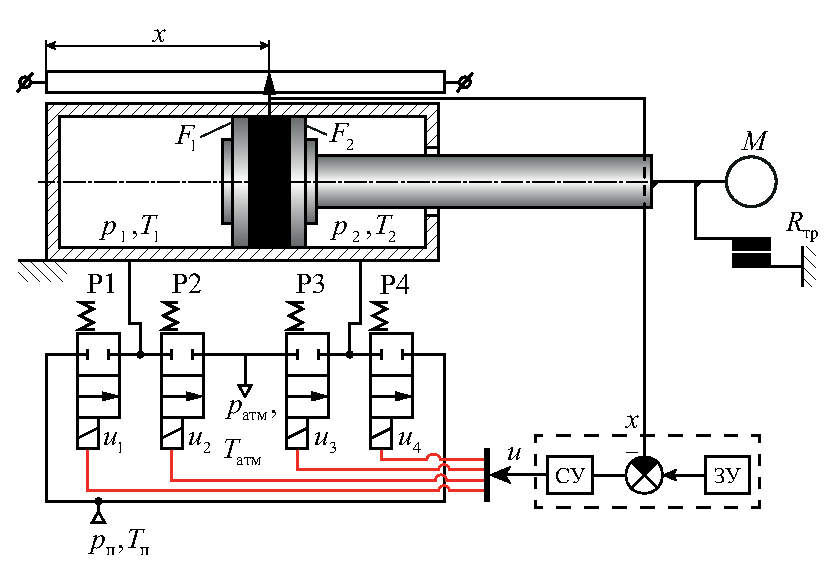
\includegraphics[width=0.85\textwidth]{Dissertation/images/part2/расчетная_схема_привода.eps}
	\caption{Схема электропневматического привода с дискретными распределителями}
	\label{fig:pneumatic_cylinder}
\end{figure}

Получено уравнение механического движения поршня с учетом всех силовых факторов:
\begin{equation}
	M\ddot{x} = p_1F_1 - p_2F_2 - p_\text{атм}(F_1 - F_2) - R_\text{тр}(\dot{x}) - R_\text{упор}(x,\dot{x}).
\end{equation}

Для моделирования нелинейных эффектов трения применена модель LuGre:
\begin{equation}
	\frac{dz}{dt} = \dot{x} - \frac{\sigma_0|\dot{x}|}{g(\dot{x})}z,\quad
	R_\text{тр} = \sigma_0z + \sigma_1\dot{z} + \sigma_2v.
\end{equation}

На основе законов термодинамики получены уравнения для изменения давлений:
\begin{equation}
	\frac{dp_i}{dt} = \frac{\gamma}{V_i}\left(RT_i(G_{i\text{вх}} - G_{i\text{вых}}) \mp p_i F_i\frac{dx}{dt}\right).
\end{equation}

Массовый расход через распределители описан с помощью закона Сен-Венана-Ванцеля:
\begin{equation}
	G = \psi(p_1, p_2) \cdot C_d F_{max} \cdot u \frac{p_1}{\sqrt{RT_\text{вх}}},
\end{equation}
где $\psi(p_1, p_2)$ -- расходная функция, определяющая режим течения газа через распределитель.

Учтена динамика переключения распределителей: $\tau du/dt + u = u_{\text{зад}}$.
Полная математическая модель представлена системой из 9 дифференциальных уравнений,
решение которой осуществляется методом обратного дифференцирования (BDF) с адаптивным шагом.
С использованием разработанной модели исследованы динамические
характеристики пневмопривода. Выявлены и классифицированы 7
основных режимов функционирования из 16 теоретически возможных комбинаций состояний распределителей:

\begin{itemize}
	\item сильного положительного ускорения [1,0,0,1];
	\item умеренного положительного ускорения [1,0,0,0];
	\item слабого положительного ускорения [0,0,0,1];
	\item сильного отрицательного ускорения [0,1,1,0];
	\item умеренного отрицательного ускорения [0,0,1,0];
	\item слабого отрицательного ускорения [0,1,0,0];
	\item удержания [0,0,0,0];
\end{itemize}

Для каждого режима получены аналитические зависимости, характеризующие
динамику давлений и движение поршня. Установлено влияние
начальных условий на характер переходных процессов. Так, в режиме
умеренного положительного ускорения выявлено, что давление в штоковой полости
изменяется согласно зависимости $p_2V_2(x)^n = \text{const}$. Для режима удержания получено линеаризованное уравнение:
\begin{equation}
	M\ddot{x} + \left(\frac{\gamma p_{1,0}F_1^2}{V_{1,0}} + \frac{\gamma p_{2,0}F_2^2}{V_{2,0}}\right)x + \nu\dot{x} = 0.
\end{equation}

Построенные фазовые портреты и полученные математические зависимости позволяют
научно обоснованно подходить к выбору режимов работы при проектировании
алгоритмов управления пневмоприводом, обеспечивая требуемые показатели качества
позиционирования при минимизации количества переключений распределителей.


\underline{\textbf{Третья глава}}
посвящена разработке и исследованию методов управления позиционным
пневмоприводом с дискретными распределителями.

Разработан модифицированный ПИД-регулятор с ШИМ, включающий блок прогнозирования
тормозного пути. Математическая модель адаптивного торможения основана на анализе кинетической энергии системы:
\begin{equation}
	s_{\text{торм}}(t) = \frac{v(t)|v(t)|}{2a_{\text{торм}}} \cdot \left(1 + K_\text{нл} \cdot e^{-\frac{|v(t)|}{v_\text{хар}}}\right),
\end{equation}
где $v(t)$ -- скорость привода;
$a_{\text{торм}}$ -- желаемое ускорение торможения;
$K_\text{нл}$ -- коэффициент нелинейности;
$v_\text{хар}$ -- характерная скорость.

Результирующее управляющее воздействие формируется как комбинация сигналов:
\begin{equation}
	u_{\text{м}}(t) = (1 - k_{\text{торм}}(t))u_{\text{пид}}(t) + k_{\text{торм}}(t)u_{\text{торм}}(t),
\end{equation}
где интенсивность торможения $k_{\text{торм}}(t)$ определяется соотношением
между прогнозируемым тормозным путем и расстоянием до целевой точки.
Данная модификация устраняет перерегулирование при сохранении приемлемой
точности позиционирования. На алгоритм получено свидетельство о регистрации программы для ЭВМ.

\begin{figure}[h]
	\centering
	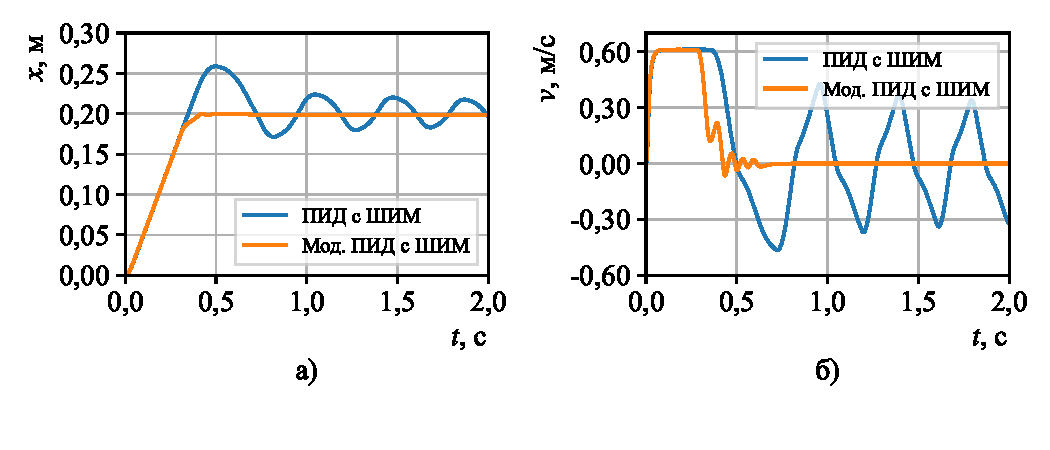
\includegraphics[width=\textwidth]{pid_comparison_2.pdf}
	\caption{Сравнение переходных процессов для классической и модифицированной структур ПИД-регулятора с ШИМ управлением}
\end{figure}

Для управления в скользящих режимах разработаны три конфигурации: трехрежимная, пятирежимная и семирежимная. Для пятирежимного управления закон имеет вид:
\begin{equation}
	\mathbf{u}(s) = \begin{cases}
		[1,0,0,1], & s > \varepsilon_2;                       \\
		[1,0,0,0], & \varepsilon_1 <   s \leq \varepsilon_2;  \\
		[0,0,0,0], & |s| \leq \varepsilon_1;                  \\
		[0,0,1,0], & -\varepsilon_2 <  s \leq -\varepsilon_1; \\
		[0,1,1,0], & s \leq -\varepsilon_2,
	\end{cases}
\end{equation}
где $s$ -- функция поверхности скольжения; $\varepsilon_1, \varepsilon_2$ -- параметры, определяющие границы зон переключения.

Исследованы две модификации поверхности скольжения: интегральная, обеспечивающая нулевую статическую ошибку:
\begin{equation}
	s_I = \dot{e} + \lambda_1 e + \lambda_2 \int_0^t e(\tau)d\tau,
\end{equation}
и терминальная, обеспечивающая конечное время сходимости:
\begin{equation}
	s_T = \dot{e} + \beta |e|^{q/p} \text{sign}(e),
\end{equation}
где $p$ и $q$ -- нечетные числа $(1 < q/p < 2)$; $\beta$ -- положительный коэффициент.

Установлено, что семирежимное управление обеспечивает наилучшее качество
позиционирования, создавая оптимальную градацию торможения.

Разработан нечеткий регулятор с двумя входными
лингвистическими переменными (ошибка позиционирования и скорость), характеризуемыми
пятью термами. База из 25 правил нечеткого вывода основывается на
знаниях физических процессов происходящих в рассматриваемом приводе.
Адаптивное изменение интенсивности
управляющего воздействия минимизирует число переключений распределителей.

Предложен оригинальный алгоритм прогнозного управления, основанный
на оптимизации на каждом шаге с использованием целевой функции:
\begin{equation}
	\begin{aligned}
		J & = \sum_{i=1}^{N_p} Q_{\text{поз}} \cdot (x(k+i|k) - x_{\text{зад}})^2 + \sum_{i=1}^{N_p} Q_{\text{скор}} \cdot v(k+i|k)^2 + \\
		  & + \sum_{i=0}^{N_c-1} R_{\text{перекл}} \cdot \sum_{j=1}^{4} |u_j(k+i|k) - u_j(k+i-1|k)|,
	\end{aligned}
\end{equation}
где $N_p$ -- горизонт прогноза; $N_c$ -- горизонт управления.

Для снижения вычислительных затрат разработан эвристический
алгоритм формирования пространства поиска, а так же упрощенная математическая модель позиционного пневмопривода.
Научно обоснованы оптимальные
значения горизонта прогноза $8 \leq N_p \leq 15$.

Проведенное исследование позволило определить преимущества и
ограничения каждого метода управления, что является основой для
выбора оптимальной структуры системы в зависимости от приоритетных требований.

\underline{\textbf{Четвертая глава}}
посвящена экспериментальной проверке разработанных математических моделей и алгоритмов
управления позиционным пневмоприводом с дискретными распределителями. Для проведения исследований
разработан специализированный лабораторный стенд, включающий пневмоцилиндр двустороннего действия с
односторонним штоком, четыре дискретных двухпозиционных распределителя, систему измерения и управления.

Экспериментальная установка реализована по иерархическому принципу и включает три основных уровня:
исполнительный уровень (датчики и актуаторы), уровень управления реального
времени (микроконтроллер STM32F767ZI) и уровень человеко-машинного
интерфейса (одноплатный компьютер Raspberry Pi 5). Система обеспечивает сбор данных с 24-битного
аналого-цифрового преобразователя с частотой дискретизации 1 кГц, реализацию
алгоритмов управления в реальном времени и визуализацию результатов через веб-интерфейс.

Программа экспериментального исследования включала следующие этапы:
\begin{enumerate}
	\item Экспериментальное определение параметров модели пневмопривода
	\item Получение и анализ экспериментальных данных о переходных процессах при различных алгоритмах управления
	\item Оценка адекватности разработанной математической модели
\end{enumerate}

Экспериментальное определение параметров модели включало тарировку потенциометрического
датчика положения Festo MLO-POT-450-TLF, измерение силы трения и времени срабатывания
распределителей. Тарировочная характеристика датчика описывается линейной зависимостью:
\begin{equation}
	x = \num{222.15}U - \num{16.00},
\end{equation}
где $x$ -- перемещение в миллиметрах, $U$ -- напряжение в вольтах.

Коэффициент детерминации $R^2 = \num{0.9998}$ подтверждает высокую линейность характеристики, а максимальная абсолютная погрешность не превышает \num{0.087} мм.
Для измерения силы трения проводились эксперименты в различных режимах: гармонические колебания,
постепенный разгон/торможение и многократные реверсы движения. Идентификация параметров модели трения
LuGre выполнялась методом наименьших квадратов с применением алгоритма Левенберга-Марквардта.
Полученные параметры
%(таблица \ref{tab1})
обеспечивают коэффициент детерминации $R^2 = \num{0.98229}$ при сравнении экспериментальной и модельной силы трения.
% \begin{table}[h]
% 	\centering
% 	\caption{Основные параметры модели трения LuGre}
% 	\label{tab1}
% 	\small
% 	\begin{tabular}{lll}
% 		\hline
% 		\textbf{Параметр} & \textbf{Значение} & \textbf{Единица измерения} \\
% 		\hline
% 		$f_c$             & \num{35.0718}     & Н                          \\
% 		$f_s$             & \num{47.1895}     & Н                          \\
% 		$v_s$             & \num{0.0151}      & \si{\metre\per\second}     \\
% 		$\sigma_0$        & \num{14280.0364}  & \si{\newton\per\metre}     \\
% 		\hline
% 	\end{tabular}
% \end{table}

Исследование времени срабатывания распределителей Camozzi A331-0C2 показало, что общее время
составляет примерно 31 мс как при открытии, так и при закрытии,
при этом стандартное квадратичное отклонение не превышает \num{2.1}~мс, что
свидетельствует о высокой повторяемости динамических характеристик.

Экспериментальное исследование переходных процессов позиционирования проводилось для четырех типов
алгоритмов управления: ПИД-регулятор с ШИМ, управление в скользящих режимах (УСР) с
различными конфигурациями, нечеткое управление и прогнозное управление. Для каждого алгоритма варьировались параметры настройки и регистрировались следующие показатели:

\begin{itemize}
	\item перемещение штока пневмоцилиндра $x(t)$;
	\item скорость движения $\dot{x}(t)$;
	\item давления в полостях пневмоцилиндра $p_1(t)$ и $p_2(t)$;
	\item комбинации состояний распределителей $\mathbf{u}(t)$;
	\item время переходного процесса $t_{\text{п}}$;
	\item статическая ошибка позиционирования $\Delta_{\text{ст}}$;
	\item перерегулирование $\sigma$;
	\item количество переключений между режимами $N_{\text{п}}$.
\end{itemize}

Сравнительный анализ экспериментальных данных (таблица \ref{tab2}) подтвердил
наличие компромисса между точностью позиционирования, быстродействием и ресурсными показателями системы.
\begin{table}[h]
	\centering
	\caption{Сравнительные характеристики алгоритмов управления}
	\label{tab2}
	\small
	\begin{tabular}{lccc}
		\hline
		\textbf{Алгоритм управления} & \textbf{Точность, мм} & \textbf{Время, с} & \textbf{Переключения} \\
		\hline
		ПИД с ШИМ                    & \num{0.60}            & \num{0.37}        & 272                   \\
		УСР-И-5                      & \num{0.62}            & \num{0.67}        & 17                    \\
		Нечеткая логика              & \num{0.95}            & \num{0.72}        & 9                     \\
		Прогнозное управление        & \num{0.80}            & \num{0.35}        & 7                     \\
		\hline
	\end{tabular}
\end{table}
ПИД-регулятор с ШИМ демонстрирует высокую частоту переключений распределителей
(272~--~527 за цикл), что негативно влияет на ресурс системы. Управление
в скользящих режимах с пятью градациями (УСР-И-5) обеспечивает хорошую точность
позиционирования (\num{0.62} мм) при значительно меньшем числе переключений (17). Нечеткое управление
характеризуется минимальным количеством переключений (9) при приемлемой точности (\num{0.95} мм).
Прогнозное управление демонстрирует оптимальное сочетание показателей: высокую точность (\num{0.80} мм),
минимальное время установления (\num{0.35} с) и наименьшее число переключений (7).
Оценка адекватности математической модели проводилась путем сравнения экспериментальных и
расчетных переходных процессов с использованием следующих метрик: коэффициент детерминации
$R^2$, среднеквадратичная ошибка $RMSE$ и относительная ошибка $\delta$. Для каждого алгоритма
управления оценивалось соответствие по четырем параметрам: перемещение штока, скорость,
давление в поршневой полости и давление в штоковой полости.

Результаты сравнительного анализа (рисцнок \ref{fig3}) показали, что разработанная математическая модель
с высокой точностью воспроизводит динамику пневмопривода для всех исследованных алгоритмов управления.
Наибольшую точность моделирования демонстрируют алгоритмы прогнозного управления (средняя относительная ошибка \num{4.36}\%)
и семирежимного управления в скользящих режимах с интегральной поверхностью (средняя ошибка \num{4.65}). Для алгоритмов
с высокой интенсивностью переключений, таких как ПИД-регулятор с ШИМ, относительная ошибка несколько выше (\num{5.87}\%).

\begin{figure}[h]
	\centering
	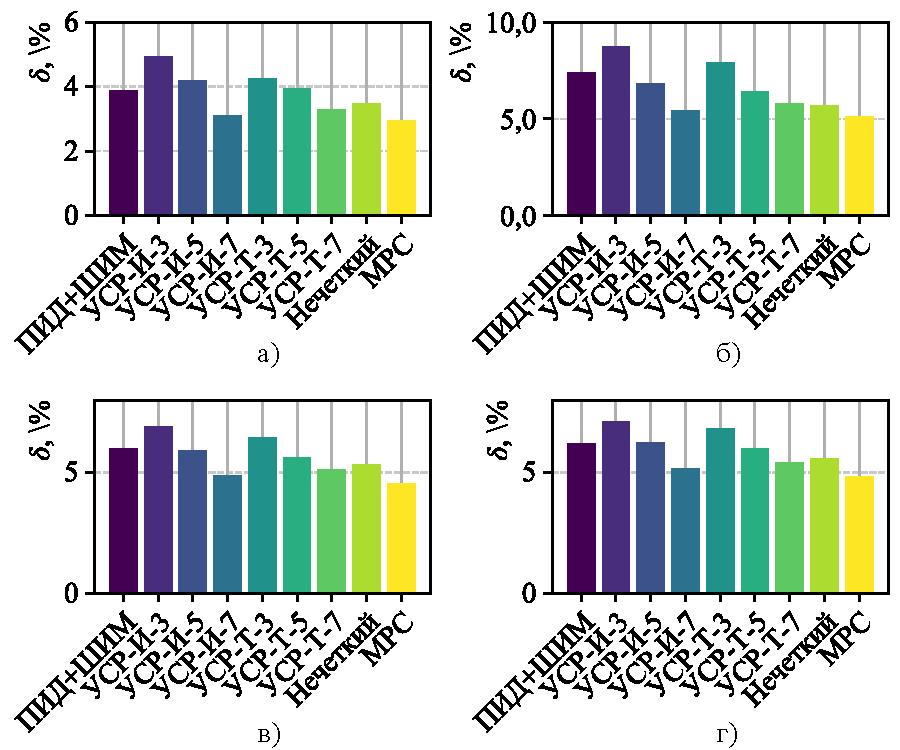
\includegraphics[width=0.9\textwidth]{Dissertation/images/part4/verification/delta_diagram.pdf}
	\caption{Сравнение точности моделирования различных алгоритмов управления по относительной ошибке $\delta$, \%\\
	а) перемещение штока; б) скорость движения; в) давление в поршневой полости; г) давление в штоковой полости}
	\label{fig3}
\end{figure}
Наиболее точно во всех случаях моделируется перемещение штока (среднее значение $R^2$ превышает \num{0.98}),
что важно для оценки точности позиционирования. Наибольшие расхождения наблюдаются при прогнозировании давлений
в полостях, что связано со сложностью моделирования термодинамических процессов.
Проведенные экспериментальные исследования подтвердили адекватность разработанной математической модели и
эффективность предложенных алгоритмов управления. Установлена высокая степень соответствия между результатами
математического моделирования и данными натурных экспериментов, что позволяет использовать разработанную методику
структурно-параметрического синтеза для оптимизации пневмоприводов с учетом требований по
точности позиционирования, быстродействию и ресурсу распределителей.

В \underline{\textbf{пятой главе}}
представлена методика многокритериального структурно-параметрического синтеза
позиционного пневмопривода с дискретными распределителями. Сформулирована задача структурно-параметрического
синтеза, включающая выбор оптимальной структуры управления и определение её параметров с учётом конфликтующих
требований к точности позиционирования, качеству переходных процессов и ресурсным показателям.

Для количественной оценки эффективности функционирования различных структур введены критерии
оптимизации: точность позиционирования ($AC$), интегральный критерий качества переходного процесса ($ITAE$) и
интенсивность переключений распределителей ($SI$), которые определяются следующими выражениями:
\begin{equation}
	AC = \lim_{t \to \infty} |e(t)| = \lim_{t \to \infty} |x_{\text{зад}} - x(t)|,
\end{equation}
\begin{equation}
	ITAE = \int_0^{T_{\text{мод}}} t |e(t)| dt,
\end{equation}
\begin{equation}
	SI = \sum_{i=1}^4 N_i,
\end{equation}
где $x_{\text{зад}}$ -- заданное положение,
$x(t)$ -- текущее положение штока,
$N_i$ -- количество переключений $i$-го распределителя.

Разработан алгоритм построения фронтов Парето, основанный на
применении замещающих суррогатных нейросетевых моделей с резидуальными блоками.
Показано, что использование метода латинского гиперкуба для формирования обучающей
выборки обеспечивает наиболее равномерное заполнение пространства параметров, что подтверждается оптимальным значением коэффициента Монте-Карло.

На основе построенных суррогатных моделей получены фронты Парето для девяти конкурсных
структур управления, включающих модифицированный ПИД-регулятор с ШИМ, управление в скользящих
режимах с различными поверхностями (интегральной и терминальной) и числом режимов (3, 5 и 7), нечёткое и прогнозное управление.

Для решения обратной задачи оптимизации разработан алгоритм поиска ближайшей
точки на фронте Парето к заданной целевой точке, основанный на нормализации критериев:
\begin{equation}
	\tilde{y}_i = \frac{y_i - y_{i,\min}}{y_{i,\max} - y_{i,\min}}, \quad i \in \{AC, ITAE, SI\},
\end{equation}
и применении взвешенной евклидовой нормы:
\begin{equation}
	\|\mathbf{\tilde{y}}(\mathbf{p}) - \mathbf{\tilde{y}}^*\|_w = \sqrt{\sum_{i} w_i (\tilde{y}_i(\mathbf{p}) - \tilde{y}_i^*)^2}.
\end{equation}

Предложенный метод коррекции параметров, базирующийся на
последовательных приближениях:
\begin{equation}
	\mathbf{p}^{(n+1)} = \mathbf{p}^{(n)} + \beta (\mathbf{y}^* - \mathbf{y}^{(n)}) \cdot \frac{\partial \mathbf{y}}{\partial \mathbf{p}}|_{\mathbf{p}^{(n)}},
\end{equation}
обеспечивает высокую точность нахождения оптимальных параметров управления.

В результате проведённого анализа фронтов Парето выделены предпочтительные
области применения различных структур управления и разработаны практические
рекомендации по их выбору. Установлено, что наивысшую точность позиционирования
(0,13~--~0,14 мм) обеспечивают семирежимное управление в скользящих режимах и прогнозное
управление, наилучшие динамические характеристики ($ITAE = \num{0,006}$ \si{\metre\per\second\square}) демонстрирует нечёткое управление, а наибольшее ресурсосбережение ($SI = 5$) -- пятирежимное управление в скользящих режимах с интегральной поверхностью.

Предложенная методика двухэтапного структурно-параметрического синтеза и сформированные
рекомендации обеспечивают возможность обоснованного выбора оптимальной
структуры пневмопривода с дискретными распределителями и определения её параметров для конкретных условий эксплуатации.


\FloatBarrier
\pdfbookmark{Заключение}{conclusion}                                  % Закладка pdf
В \underline{\textbf{заключении}} приведены основные результаты работы, которые заключаются в следующем:

\begin{enumerate}
	\item Разработана комплексная математическая модель позиционного пневмопривода с дискретными распределителями,
	      которая включает в себя как силовую, так и управляющую структуры. Модель учитывает нелинейные термодинамические
	      процессы в полостях пневмоцилиндра, переменную структуру системы при переключении распределителей, а также
	      динамические эффекты сухого и вязкого трения. Высокая степень согласованности результатов моделирования с
	      экспериментальными данными (расхождение не превышает 5~--~7\%) подтверждает адекватность и достоверность
	      разработанной модели для решения задач анализа и синтеза пневмоприводов различной структуры.

	\item Проведен комплексный анализ различных структур пневмопривода, что позволило выявить оптимальные
	      режимы переключения распределителей при позиционировании рабочего органа. Разработаны структуры управления
	      на основе различных принципов: модифицированная структура ПИД-регулятора с блоком прогнозирования тормозного пути,
	      управление в скользящих режимах с интегральной и терминальной поверхностями, нечеткое управление и прогнозное управление.
	      Экспериментальный анализ подтвердил, что прогнозное управление обеспечивает повышение точности позиционирования на 25~--~30\%
	      при одновременном сокращении числа переключений распределителей на 35~--~45\% по сравнению с традиционными алгоритмами.

	\item Проведен натурный эксперимент на специально разработанном лабораторном стенде, который подтвердил работоспособность
	      предложенных структур и высокую достоверность результатов, полученных с использованием разработанной математической модели.
	      Сравнительный анализ экспериментальных данных показал, что наибольшую точность моделирования демонстрируют алгоритмы прогнозного
	      управления и семирежимного управления в скользящих режимах, где средняя относительная ошибка не превышает 4,65\%.
	      Расхождение между расчетными и экспериментальными данными по основным показателям качества составляет
	      не более 7\% для всех исследованных алгоритмов управления.

	\item Разработана методика многокритериального структурно-\allowbreak па\-ра\-ме\-три\-че\-ско\-го синтеза, основанная
	      на использовании фронтов Парето с применением замещающей суррогатной нейросетевой модели. Для
	      формирования обучающей выборки применен метод латинского гиперкуба, обеспечивающий оптимальное
	      заполнение пространства параметров, что позволило сократить вычислительные затраты при построении
	      фронтов Парето на 48\%. Использование суррогатной модели обеспечило среднюю точность аппроксимации 91\%
	      при максимальном отклонении 12\%.

	\item Определена взаимосвязь между конфликтными статико-динамическими и ресурсными показателями
	      для позиционных пневмоприводов различной структуры на основе анализа фронтов Парето. Установлено,
	      что для ПИД-регулятора с ШИМ диапазон изменения критерия $ITAE$ составляет от 0,0298 до 0,0427 \si{\meter\per\second\square}
	      при изменении точности от 0,41 до 2,57 мм. Семирежимное управление с интегральной поверхностью
	      обеспечивает точность 0,13 мм при $ITAE = 0,019$ \si{\meter\per\second\square} и $SI = 15$, а прогнозное управление демонстрирует
	      точность 0,12 мм при $ITAE = 0,032$ \si{\meter\per\second\square} и $SI = 14$~--~$16$. Для нечеткого регулятора характерны
	      наилучшие показатели по критерию динамической эффективности ($ITAE = 0,006$ \si{\meter\per\second\square}) при точности 0,40 мм.

	\item Сформированы практические рекомендации по выбору оптимальной структуры позиционного
	      пневмопривода с дискретными распределителями. Выделены четыре предпочтительные области
	      применения различных алгоритмов управления:
	      \begin{itemize}
		      \item область высоконагруженных систем (УСР-И-5, MPC) с точностью 0,12~--~0,36 мм;
		      \item область точных манипуляторов (УСР-И-7) с точностью 0,14 мм;
		      \item область промышленной автоматики (УСР-Т-5, УСР-Т-7) с точностью 0,13~--~0,28 мм;
		      \item область простых систем (ПИД+ШИМ, УСР-И-3) с точностью 0,5~--~2,5 мм.
	      \end{itemize}
	      Определены рекомендуемые значения параметров алгоритмов управления для типовых задач
	      позиционирования, что позволяет сократить сроки проектирования и повышает эффективность разрабатываемых систем.
\end{enumerate}

Полученные результаты позволяют на научной основе выбирать оптимальную структуру и
параметры позиционного пневмопривода с дискретными распределителями в зависимости
от конкретных требований, существенно сокращая сроки проектирования и повышая
эффективность разрабатываемых систем.

% %% Согласно ГОСТ Р 7.0.11-2011:
%% 5.3.3 В заключении диссертации излагают итоги выполненного исследования, рекомендации, перспективы дальнейшей разработки темы.
%% 9.2.3 В заключении автореферата диссертации излагают итоги данного исследования, рекомендации и перспективы дальнейшей разработки темы.
В результате проведенного диссертационного исследования достигнута поставленная
цель комплексного повышения статико-динамических и ресурсных показателей позиционного пневмопривода с
дискретными распределителями в условиях их конфликтности. Получены следующие основные результаты:

\begin{enumerate}
    \item Разработана комплексная математическая модель позиционного пневмопривода с дискретными распределителями,
    которая включает в себя как силовую, так и управляющую структуры. Модель учитывает нелинейные термодинамические
    процессы в полостях пневмоцилиндра, переменную структуру системы при переключении распределителей, а также
    динамические эффекты сухого и вязкого трения. Высокая степень согласованности результатов моделирования с
    экспериментальными данными (расхождение не превышает 5~--~7\%) подтверждает адекватность и достоверность
    разработанной модели для решения задач анализа и синтеза пневмоприводов различной структуры.

    \item Проведен комплексный анализ различных структур пневмопривода, что позволило выявить оптимальные
    режимы переключения распределителей при позиционировании рабочего органа. Разработаны структуры управления
    на основе различных принципов: модифицированная структура ПИД-регулятора с блоком прогнозирования тормозного пути,
    управление в скользящих режимах с интегральной и терминальной поверхностями, нечеткое управление и прогнозное управление.
    Экспериментальный анализ подтвердил, что прогнозное управление обеспечивает повышение точности позиционирования на 25~--~30\%
    при одновременном сокращении числа переключений распределителей на 35~--~45\% по сравнению с традиционными алгоритмами.

    \item Проведен натурный эксперимент на специально разработанном лабораторном стенде, который подтвердил работоспособность
    предложенных структур и высокую достоверность результатов, полученных с использованием разработанной математической модели.
    Сравнительный анализ экспериментальных данных показал, что наибольшую точность моделирования демонстрируют алгоритмы прогнозного
    управления и семирежимного управления в скользящих режимах, где средняя относительная ошибка не превышает 4,65\%.
    Расхождение между расчетными и экспериментальными данными по основным показателям качества составляет
    не более 7\% для всех исследованных алгоритмов управления.

    \item Разработана методика многокритериального структурно-параметрического синтеза, основанная
    на использовании фронтов Парето с применением замещающей суррогатной нейросетевой модели. Для
    формирования обучающей выборки применен метод латинского гиперкуба, обеспечивающий оптимальное
    заполнение пространства параметров, что позволило сократить вычислительные затраты при построении
    фронтов Парето на 48\%. Использование суррогатной модели обеспечило среднюю точность аппроксимации 91\%
    при максимальном отклонении 12\%.

    \item Определена взаимосвязь между конфликтными статико-динамическими и ресурсными показателями
    для позиционных пневмоприводов различной структуры на основе анализа фронтов Парето. Установлено,
    что для ПИД-регулятора с ШИМ диапазон изменения критерия $ITAE$ составляет от 0,0298 до 0,0427 \si{\meter\per\second\square}
    при изменении точности от 0,41 до 2,57 мм. Семирежимное управление с интегральной поверхностью
    обеспечивает точность 0,13 мм при $ITAE = 0,019$ \si{\meter\per\second\square} и $SI = 15$, а прогнозное управление демонстрирует
    точность 0,12 мм при $ITAE = 0,032$ \si{\meter\per\second\square} и $SI = 14$~--~$16$. Для нечеткого регулятора характерны
    наилучшие показатели по критерию динамической эффективности ($ITAE = 0,006$ \si{\meter\per\second\square}) при точности 0,40 мм.

    \item Сформированы практические рекомендации по выбору оптимальной структуры позиционного
    пневмопривода с дискретными распределителями. Выделены четыре предпочтительные области
    применения различных алгоритмов управления:
    \begin{itemize}
        \item область высоконагруженных систем (УСР-И-5, MPC) с точностью 0,12~--~0,36 мм;
        \item область точных манипуляторов (УСР-И-7) с точностью 0,14 мм;
        \item область промышленной автоматики (УСР-Т-5, УСР-Т-7) с точностью 0,13~--~0,28 мм;
        \item область простых систем (ПИД+ШИМ, УСР-И-3) с точностью 0,5~--~2,5 мм.
    \end{itemize}
    Определены рекомендуемые значения параметров алгоритмов управления для типовых задач
    позиционирования, что позволяет сократить сроки проектирования и повышает эффективность разрабатываемых систем.
\end{enumerate}

Полученные результаты позволяют на научной основе выбирать оптимальную структуру и
параметры позиционного пневмопривода с дискретными распределителями в зависимости
от конкретных требований, существенно сокращая сроки проектирования и повышая
эффективность разрабатываемых систем.

\pdfbookmark{Литература}{bibliography}                                % Закладка pdf
% При использовании пакета \verb!biblatex! список публикаций автора по теме
% диссертации формируется в разделе <<\publications>>\ файла
% \verb!common/characteristic.tex!  при помощи команды \verb!\nocite!

\ifdefmacro{\microtypesetup}{\microtypesetup{protrusion=false}}{} % не рекомендуется применять пакет микротипографики к автоматически генерируемому списку литературы
\urlstyle{rm}                               % ссылки URL обычным шрифтом
\ifnumequal{\value{bibliosel}}{0}{% Встроенная реализация с загрузкой файла через движок bibtex8
	\renewcommand{\bibname}{\large \bibtitleauthor}
	\nocite{*}
	\insertbiblioauthor           % Подключаем Bib-базы
	%\insertbiblioexternal   % !!! bibtex не умеет работать с несколькими библиографиями !!!
}{% Реализация пакетом biblatex через движок biber
	% Цитирования.
	%  * Порядок перечисления определяет порядок в библиографии (только внутри подраздела, если `\insertbiblioauthorgrouped`).
	%  * Если не соблюдать порядок "как для \printbibliography", нумерация в `\insertbiblioauthor` будет кривой.
	%  * Если цитировать каждый источник отдельной командой --- найти некоторые ошибки будет проще.
	%
	%% authorvak
	\nocite{vakbib1}%
	\nocite{vakbib2}%
	\nocite{vakbib3}%
	\nocite{vakbib4}%
	\nocite{vakbib5}%
	\nocite{vakbib6}%
	\nocite{vakbib7}%
	\nocite{vakbib8}%
	\nocite{vakbib9}%
	\nocite{vakbib10}%
	\nocite{vakbib11}%
	\nocite{vakbib12}%
	\nocite{pub4}%
	\nocite{pub21}%
	\nocite{pub22}%
	%
	%% authorwos
	\nocite{wosbib1}%
	%
	%% authorscopus
	\nocite{scbib1}%
	%
	%% authorpatent
	\nocite{patbib1}%
	%
	%% authorprogram
	\nocite{progbib1}%
	%
	%% authorconf
	\nocite{pub3}
	\nocite{pub8}
	\nocite{pub13}
	\nocite{pub14}
	\nocite{pub16}
	\nocite{pub19}
	\nocite{pub20}
	%
	%% authorother
	\nocite{pub6}%


	\ifnumgreater{\value{usefootcite}}{0}{
		\begin{refcontext}[labelprefix={}]
			\ifnum \value{bibgrouped}>0
				\insertbiblioauthorgrouped    % Вывод всех работ автора, сгруппированных по источникам
			\else
				\insertbiblioauthor      % Вывод всех работ автора
			\fi
		\end{refcontext}
	}{
		\ifnum \totvalue{citeexternal}>0
			\begin{refcontext}[labelprefix=A]
				\ifnum \value{bibgrouped}>0
					\insertbiblioauthorgrouped    % Вывод всех работ автора, сгруппированных по источникам
				\else
					\insertbiblioauthor      % Вывод всех работ автора
				\fi
			\end{refcontext}
		\else
			\ifnum \value{bibgrouped}>0
				\insertbiblioauthorgrouped    % Вывод всех работ автора, сгруппированных по источникам
			\else
				\insertbiblioauthor      % Вывод всех работ автора
			\fi
		\fi
		%  \insertbiblioauthorimportant  % Вывод наиболее значимых работ автора (определяется в файле characteristic во второй section)
		\begin{refcontext}[labelprefix={}]
			\insertbiblioexternal            % Вывод списка литературы, на которую ссылались в тексте автореферата
		\end{refcontext}
		% Невидимый библиографический список для подсчёта количества внешних публикаций
		% Используется, чтобы убрать приставку "А" у работ автора, если в автореферате нет
		% цитирований внешних источников.
		\printbibliography[heading=nobibheading, section=0, env=countexternal, keyword=biblioexternal, resetnumbers=true]%
	}
}
\ifdefmacro{\microtypesetup}{\microtypesetup{protrusion=true}}{}
\urlstyle{tt}                               % возвращаем установки шрифта ссылок URL
      % Содержание автореферата

%%% Выходные сведения типографии
\newpage\thispagestyle{empty}

\vspace*{0pt plus1fill}

\small
\begin{center}
    \textit{\thesisAuthor}
    \par\medskip

    \thesisTitle
    \par\medskip

    Автореф. дис. на соискание ученой степени \thesisDegreeShort
    \par\bigskip

    Подписано в печать \blank[\widthof{999}].\blank[\widthof{999}].\blank[\widthof{99999}].
    Заказ № \blank[\widthof{999999999999}]

    Формат 60\(\times\)90/16. Усл. печ. л. 1. Тираж 100 экз.
    %Это не совсем формат А5, но наиболее близкий, подробнее: http://ru.wikipedia.org/w/index.php?oldid=78976454

    Типография \blank[0.5\linewidth]
\end{center}
\cleardoublepage

\end{document}
